%%%%%%%%%%%%%%%%%%%%%%%%%%%%%%%%%%%%%%%%%%%%%%%%%%%%%%%%%%%%%%%%%%%%%%%%%%%%%%%%%%%%%%%%%%%%%%%%%%
% Frontiers in Microbiology MAIN manuscript (Vancouver / numbered reference style)
% Main text keeps 6 figures + 9 tables = 15 (the Frontiers limit). All other items move to
% frontiers_SupplementaryMaterial.tex and are cited here as Supplementary Table/Figure Sx.
% Compile on Overleaf/TeX Live: pdflatex -> bibtex -> pdflatex x2.
%%%%%%%%%%%%%%%%%%%%%%%%%%%%%%%%%%%%%%%%%%%%%%%%%%%%%%%%%%%%%%%%%%%%%%%%%%%%%%%%%%%%%%%%%%%%%%%%%%

\documentclass[utf8]{FrontiersinVancouver}
\usepackage{url,lineno,microtype,hyperref}
\graphicspath{{figures/}}
\linenumbers

\def\keyFont{\fontsize{8}{11}\helveticabold}
\def\firstAuthorLast{Hou}
\def\Authors{Yuan Hou$^{1}$, Haoran Gu$^{3}$, Xingshun Song$^{2,*}$ and Yan Miao$^{3,*}$}
\def\Address{$^{1}$Aulin College, Northeast Forestry University, Harbin, Heilongjiang, China \\
$^{2}$College of Life Science, Northeast Forestry University, Harbin, Heilongjiang, China \\
$^{3}$School of Computer Science and Artificial Intelligence, Northeast Forestry University, Harbin, Heilongjiang, China}
\def\corrAuthor{Xingshun Song and Yan Miao}
\def\corrEmail{[corresponding institutional emails to be supplied before submission]}

\begin{document}
\onecolumn
\firstpage{1}

\title{Neighbor leakage and ORF-derived coding signals in alignment-free phage-host prediction: a controlled benchmark}

\author[\firstAuthorLast]{\Authors}
\address{}
\correspondance{}
\extraAuth{}
\maketitle

\begin{abstract}
\section{}
\textbf{Motivation:} Alignment-free models rank bacterial hosts from phage nucleotide sequences, but their evidence is weakened by sequence-level splits that place near-identical phages in both training and test sets and by single-run comparisons. \textbf{Results:} We curate two benchmarks from public resources, CHERRY (1,875 phages, 206 hosts) and DeepHost (2,845 phages, 108 hosts), and compare deep sequence models, four classical classifiers, and an ORF-derived coding-feature encoder under a random and a similarity-aware split, over five seeds. The data partition is the largest effect: the full model falls from 74.68\% to 44.92\% top-1 accuracy (29.76 points; Holm-adjusted $p=0.0033$). A logistic regression on the same FCGR features reaches 82.3\% and 83.6\%, matching or exceeding every deep model. A phage-level paired bootstrap and sign-flip permutation show that the architectural components do not give a stable gain: the bidirectional Mamba2 block does not improve ranking on a fixed split, while in an exploratory fixed-split analysis the genuine FCGR signal is higher than a permuted representation under the similarity split (unadjusted permutation $p=0.043$). A uniform validation-set grid search confirms that the published classical-model defaults are already adequate for logistic regression, random forest, and the support vector machine (mean absolute change 2.29 points), with only k-nearest neighbors sensitive to its neighbor count. ORF-derived coding features outperform FCGR; the strongest contrasts survive family-wise correction across a single, explicitly defined family of 13 tests (Holm $p$ as low as 0.0082), whereas borderline contrasts hold under false-discovery-rate control but not under the stricter Holm procedure. This signal is not explained by GC content, sequence length, or gene count: codon frequencies retain their accuracy after residualization against GC, while a GC/length/gene-count baseline reaches only 39\%. Host-phylogeny controls that use the real genus label are kept strictly post-hoc and never enter the deployed predictor, which uses only sequence-derived features. Because the two resources overlap substantially (767 shared phage accessions; 85.5\% of CHERRY phages have a cosine $\geq$0.999 DeepHost neighbor) and cross-dataset accuracy collapses after sequence de-duplication (91.1\% to 19.2\% in the strongest direction), we do not treat the second dataset as independent external validation. Temperature scaling lowers mean expected calibration error from 0.729 to 0.067, and a calibrated confidence detects withheld hosts (AUROC 0.91--0.94). We describe codon usage as predictive and consistent with, but not proof of, translational adaptation. \textbf{Availability:} the code, processed data, and per-run results are provided in the reproducibility package and in the public repository \url{https://github.com/QWERasd12345-ASD/BMKMPHI}.

\tiny
\keyFont{\section{Keywords:} phage-host prediction, data leakage, similarity-aware split, classical machine-learning baselines, ORF-derived coding features, codon usage, confidence calibration}
\end{abstract}

\section{Introduction}

Bacteriophages are viruses that infect bacteria and are among the most abundant biological entities in microbial communities. Their host ranges are typically narrow, and infection can reshape bacterial population structure, horizontal gene transfer, and processes linked to disease. Assigning a bacterial host to a phage sequence recovered from a metagenomic sample is therefore a central step in viral ecology and in phage-based applications.

Experimental host assignment through culturing is low-throughput and expensive, so computational methods dominate at scale. Alignment-based tools exploit homology, and CRISPR-spacer or receptor-binding protein approaches use specific molecular evidence, but these depend on reference completeness or on a recognizable immune record. Alignment-free methods instead encode sequence composition---k-mer frequencies, oligonucleotide usage, or frequency chaos game representation (FCGR)~\citep{wang2026phagecgrnet}---and learn a mapping from phage to host, often with a contrastive or classification objective~\citep{guo2017equivalence}.

Two methodological problems weaken the evidence for many alignment-free models. First, benchmarks commonly split individual sequences randomly after removing only exact duplicates. Closely related phages, and fragments derived from the same genome, can then occur in both training and test sets, and a model can succeed by retrieving a near neighbor rather than by learning a generalizable host signal. Second, architectural contributions are often demonstrated with single runs and point estimates, without repeated seeds, confidence intervals, paired significance tests, or multiple-comparison correction, and with baselines reimplemented under unequal settings. It is then difficult to distinguish genuine advances from variation driven by initialization, negative sampling, or the partition itself.

These concerns are not hypothetical. In the FCGR pipeline that motivates this work, whole-genome gains over the closest competing method are small, and the difference between FCGR and a randomly permuted k-mer layout is typically below one percentage point, suggesting that k-mer composition rather than two-dimensional topology carries the discriminative signal. To our knowledge, no controlled study has simultaneously quantified neighbor leakage, benchmarked simple classifiers against deep architectures, tested whether a biologically different representation can improve host ranking under a leakage-controlled split, and checked whether that signal is confounded by simple sequence composition.

We make three contributions. (1) We build two versioned, checksum-verified benchmarks and quantify neighbor leakage with a similarity-aware split and a multi-seed threshold sweep, paired across models, with Holm and Benjamini--Hochberg correction over a documented family. (2) We derive coding features from predicted open reading frames, test whether they outperform FCGR under leakage control, and explicitly evaluate GC, length, and gene-count confounding. (3) We provide multi-seed calibration, open-set rejection, per-class and imbalance analysis, and an efficiency protocol, delineating both the validity and the limits of each representation.

\section{Materials and Methods}

\subsection{Benchmark datasets and curation audit}

We use two public resources so that conclusions can be examined across more than one data source; Table~\ref{tab:1} summarizes their statistics. The CHERRY release~\citep{shang2022cherry} provides phage nucleotide sequences and matched candidate bacterial genomes. We re-ran the original curation table rather than trusting downstream counts. Of 2,097 raw phage-host pairs, 222 lack a usable sequence and 157 carry an empty host-species field; 142 of the empty-species records still contain a genus label. We apply one explicit rule: only species-level labels are used, and empty-species or genus-only records never enter training as positives, so no genus fallback is applied. This retains 1,875 phages mapped to 206 host species across 135 genera, with zero multi-label phages, 88 singleton classes, and 59 classes containing at least five phages. The largest class is \textit{Mycolicibacterium smegmatis} (312 phages), followed by \textit{Escherichia coli} (226) and \textit{Pseudomonas aeruginosa} (117). Taxonomy is updated to current names, including the reclassification of \textit{Mycobacterium smegmatis} to \textit{Mycolicibacterium smegmatis}.

The DeepHost reference taxonomy~\citep{wang2022deephost} defines 118 standardized host species. Its processed release contains 3,567 phage sequences annotated against 366 raw host-name strings. We map each raw name to the standardized taxonomy and retain only phages whose host matches a standardized class exactly, yielding 2,845 phages over 108 occupied classes. Ten classes are empty and are excluded from the candidate set; we report them rather than silently dropping them. Outdated names are updated to current taxonomy, including \textit{Cutibacterium acnes} and \textit{Clostridioides difficile}.

To make the data version auditable, every processed file is recorded with its byte size and SHA-256 digest in a machine-readable manifest (13 files), and the host reference genomes are listed with class identifier, scientific name, accession, and sequence length. The identical encoding, features, splitting, and objective are applied to both datasets, so the benchmarks differ only in the underlying data.

\subsection{Sequence and ORF-derived coding representations}

Each nucleotide sequence is encoded with FCGR at $k=6$. The chaos-game walk maps the four bases to the corners of a unit square and, at each position $t$, moves halfway from the current point to the corner for the base $s_t$. Coordinates are binned into a $64\times64$ grid whose 4,096 cells correspond one-to-one to the 4,096 possible 6-mers. For a sequence of length $L$, let $c_m$ be the number of length-$k$ windows whose 6-mer is $m$; windows containing an ambiguous base $N$ are not counted, while the denominator remains $L-k+1$. The cell value is then
\begin{equation}
f_m = \frac{c_m}{L-k+1}
\label{eq:1}
\end{equation}
No reverse-complement merging is applied. To separate k-mer composition from the two-dimensional layout, a permuted control keeps the same 4,096 frequencies but rearranges them with a fixed, reproducible permutation before reshaping, so the frequency content is identical while the FCGR topology is removed.

Open reading frames are predicted with pyrodigal~\citep{larralde2022pyrodigal}, a Cython binding and interface to the Prodigal gene-finder~\citep{hyatt2010prodigal} that implements the Prodigal dynamic-programming algorithm rather than a pure-Python reimplementation. We construct the finder with \texttt{pyrodigal.GeneFinder(meta=True)}, running it in metagenomic mode with the default bacterial translation table 11, and pin the library version in the requirements file. The finder is called separately on every contig, so gene calls cannot span a contig boundary. Partial genes are retained and counted; overlapping ORFs are counted independently without de-duplication. The three in-frame stop codons TAA, TAG, and TGA are part of the 64 ACGT codon bins and are counted, whereas any codon containing an ambiguous base N has no index in the 64-bin table and is skipped. Predicted ORFs are translated to proteins, from which we construct a 96-dimensional vector in four blocks. The structural block (indices 0--7) contains log gene count, coding density, mean and SD of ORF length, fraction of forward-strand ORFs, fraction of complete genes, overlap fraction, and mean intergenic length. The codon block (indices 8--71) contains 64 relative codon frequencies. The amino-acid block (indices 72--91) contains 20 relative amino-acid frequencies. The physicochemical block (indices 92--95) contains mean Kyte--Doolittle hydrophobicity and the fractions of basic, acidic, and sulfur-containing residues. Each codon frequency is the count of that codon divided by the total number of codons across all predicted ORFs in the genome, so the 64 values sum to one. Coding features are standardized using the training-set mean and SD.

\subsection{Host reference genomes: selection, assembly level, and quality control}

DeepHost does not ship host genomes, so we obtained one pinned reference assembly per taxonomy class from NCBI under an explicit, documented rule. For each species we select a single RefSeq representative, preferring chromosome-sized sequences of at least 200 kb and, where several qualify, the longest such record. Whole-genome shotgun entries are represented by multiple contigs; for gene calling we process each contig independently rather than joining them, so no predicted ORF can cross a contig boundary. Of the 118 taxonomy classes, 108 carry a sequence; 104 are complete genomes and four are contig-level assemblies, giving $104+4=108$. Two of those four are multi-contig, the most fragmented being \textit{Streptomyces viridochromogenes} (757 contigs, N50 18,965 bp) and \textit{Streptomyces azureus} (86 contigs, N50 228,249 bp); the other two contig-level records (class 92 and class 97) each consist of a single contig annotated at the contig level rather than as a complete genome.

Because no contamination-model tool such as CheckM was run, we apply a transparent sequence-level screen instead and report its limits. Every assembly is checked for the ambiguous-base fraction, the presence of symbols outside the ACGT alphabet, and a robust z-score of ORF density. Across the 108 genomes the median density is 938.86 genes per Mb. Three records are flagged rather than silently removed: \textit{Vibrio parahaemolyticus} (class 26; 13.33\% ambiguous bases, 1,203 non-ACGTN symbols, 787.9 genes/Mb), \textit{Lactobacillus gasseri} (class 111; 7,842 non-ACGTN symbols), and \textit{Burkholderia thailandensis} (class 115; 5.20\% ambiguous bases). We retain these classes with an explicit flag so that any downstream effect can be traced.

\subsection{Model architecture and the two independent training pipelines}

We name the proposed model BMKMPHI [full expansion to be supplied by the authors before submission]. Its sequence encoder applies two convolutional layers (kernel size 7, stride 2; batch normalization and ReLU; max pooling after the second layer; channels 64 then 128) to the $64\times64$ matrix, followed by a bidirectional Mamba2 block over the flattened spatial tokens and a fully connected head producing a 512-dimensional embedding. The bidirectional Mamba2 block pads the token grid to a multiple of eight, runs one forward and one reverse Mamba2 layer, and sums their two outputs before cropping back to the original grid. A CNN-only variant removes this block. The coding encoder is a multilayer perceptron (96 to 256 to 256 to 512). The fusion model encodes both views, projects the coding branch to 128 dimensions, concatenates it with the 512-dimensional sequence embedding, and maps the 640-dimensional vector back to 512. Phages and candidate hosts share the same encoder in every variant. We also include an equivalent reimplementation of the published PhageCGRNet three-channel architecture~\citep{wang2026phagecgrnet}. The fixed architecture is listed in Supplementary Table~S1.

A single configuration file cannot represent two different training objectives, so the architecture and the training target are deliberately separated. One shared architecture specification (\texttt{method\_config.json}) fixes the layers and feature blocks, and two independent pipeline files specify how the network is trained. The default contrastive pipeline (\texttt{pipeline\_contrastive.json}) attaches no classification head, trains the 512-dimensional embedding with the matrix contrastive loss, ranks hosts by Euclidean distance (smaller is better), and applies three BatchNorm recalibration passes before evaluation. The separate cross-entropy pipeline (\texttt{pipeline\_ce.json}) adds a Linear(512, $n_{\text{hosts}}$) head, trains with a full-host softmax cross-entropy, ranks by logits (larger is better), and does not perform BatchNorm recalibration. Every run record names the pipeline file it used, so the two objectives are never conflated (Supplementary Table~S2).

\subsection{Splitting protocols and component allocation}

The random split assigns individual sequences to training, validation, and test sets at an 8:1:1 ratio. For leakage control we additionally build a similarity-aware split. MinHash signatures~\citep{broder1997resemblance} ($k=21$, sketch size 1,000, following Mash defaults~\citep{ondov2016mash}) are converted from pairwise Jaccard similarity to a Mash distance. Phages connected at a Mash distance no greater than 0.05, approximately 95\% average nucleotide identity, are joined into connected components, and each component is assigned as a whole to one split with a deterministic, seed-controlled allocation that preserves the 8:1:1 size ratio. At 0.05 this produces 1,049 components for CHERRY (largest 38; 793 singletons) and 1,343 for DeepHost (largest 52; 938 singletons). Because no two phages above the identity threshold cross splits, the test set cannot be solved by retrieving a near-identical training neighbor.

Component allocation has a cost that we report explicitly. Because a component cannot be divided, the classes are not evenly covered: under the CHERRY seed-123 split, 21 of the 80 test classes are absent from the training set entirely, and two of the 79 DeepHost test classes are absent. A model cannot learn these classes from training data, so the similarity-split decline reflects both the removal of neighbor leakage and uneven class coverage. We therefore avoid attributing the entire gap to leakage.

\subsection{Training objectives}

Each contrastive batch contains $B$ phages and re-encodes the full set of $J$ candidate hosts, then forms the $B\times J$ matrix of pairwise Euclidean distances. Recorded pairs are positives and label-mismatched pairs are proxy negatives, denoting the absence of a recorded interaction rather than confirmed non-infection. Let $z_i$ be phage $i$'s embedding ($i=1\ldots B$), $h_j$ host $j$'s embedding ($j=1\ldots J$), $d_{ij}=\|z_i-h_j\|$, let $y_i$ be phage $i$'s recorded host, and let the margin $m=1$. The matrix contrastive loss is
\begin{equation}
L=\frac{1}{2BJ}\sum_{i=1}^{B}\sum_{j=1}^{J}\left[\mathbf{1}[j=y_i]\,d_{ij}^{2}+\mathbf{1}[j\neq y_i]\,\big(\max(0,m-d_{ij})\big)^2\right]
\label{eq:2}
\end{equation}
The indexing and normalization make the loss fully specified. The double sum runs over every one of the $B\times J$ phage-host pairs, so all label-mismatched pairs enter the loss, not only pairs within the mini-batch. Each phage has exactly one positive, its recorded host $y_i$, and $J-1$ proxy negatives; because the candidate set is fixed, every phage has the same number of negatives. There is no separate positive or negative weight: the single factor $1/(2BJ)$ averages over all entries, matching the implementation, which takes the mean over the $B\times J$ matrix and then divides by two. The positive-negative imbalance (one versus $J-1$) is therefore not explicitly rebalanced, and the hinge terms dominate numerically.

The cross-entropy pipeline instead applies a fair full-host softmax over all candidate hosts, rather than the defective single-negative binary objective in the original study. Both pipelines are optimized with Adam at a learning rate of 1e-3 with no weight decay; the sequence benchmark runs 120 epochs and the representation comparison 100 epochs. The checkpoint with the highest validation accuracy is retained. In the contrastive pipeline, batch-normalization statistics are re-estimated on the training set before final evaluation without changing the weights.

\subsection{Metrics, correction family, and resampling}

We report top-1 and top-5 accuracy, mean reciprocal rank, macro-averaged F1, and balanced accuracy, the last being the mean per-class recall that gives equal weight to rare classes. Every primary comparison is repeated over the fixed seeds 123, 2024, 42, 7, and 99; architecture ablations use three seeds. Seeds quantify training stability under different initializations and data orders; they are not independent biological replicates. We therefore label the seed-level paired t-tests and their standardized effect size Cohen's d~\citep{cohen1988statistical} as stability descriptions rather than population-level claims. Because the smallest exact two-sided Wilcoxon p with five seeds is 0.0625, we use the sign of all five paired differences only as a robustness check.

All hypothesis tests are assigned to one explicitly defined correction family so that the adjusted p values can be reproduced from the table. The study uses a single global family of $m=13$ tests: twelve paired representation contrasts (FCGR, protein, and fusion across two datasets and two splits) plus the full-model random-versus-similarity leakage contrast. Within this family the Holm step-down procedure~\citep{holm1979simple} controls the family-wise error rate and the Benjamini--Hochberg (BH) step-up procedure~\citep{benjamini1995controlling} controls the false discovery rate. The complete list, with the rank, the unrounded raw p to six decimals, and both adjusted values, is released as \texttt{correction\_full\_list.csv} and summarized in Table~\ref{tab:6}; recomputing Holm and BH from these raw values reproduces every reported number.

To obtain inference at the phage level rather than across the handful of seeds, we add a paired bootstrap~\citep{efron1979bootstrap} and a sign-flip permutation on the same test phages. For a fixed split we record whether each test phage is correct under two models, resample the paired indicators 2,000 times with replacement, and report the percentile 95\% interval for the mean difference. The sign-flip permutation randomly reverses the within-phage model labels 2,000 times to build a null distribution for the observed difference. This pairs the two predictions on exactly the same phages, so the comparison is not confounded by a changing test set. We distinguish a non-significant result, which means the present data do not provide evidence for an effect, from evidence that no effect exists; with few seeds these are not equivalent.

\subsection{Classical baselines and a uniform tuning sensitivity}

We add four scikit-learn~\citep{pedregosa2011scikit} classifiers on the flattened FCGR (4,096 dimensions) and coding (96 dimensions) features: logistic regression (L2, $C=1$, up to 3,000 iterations, random forest (300 trees), k-nearest neighbors ($k=10$), and a radial-basis support vector machine ($C=1$). All features use a StandardScaler fitted on the training partition, and probability columns are mapped back to global class identifiers so rare-class handling cannot misalign the ranking. To test whether the published defaults are adequate, we run one uniform validation-set grid: for each model family every candidate is trained on the training partition and chosen by validation top-1, after which the default and the selected model are scored on the same test set. The grids cover the regularization strength for logistic regression, tree count and depth for the forest, the neighbor count for k-nearest neighbors, and the cost and kernel width for the support vector machine.

\subsection{Calibration and open-set rejection}

A single temperature parameter is fitted on the validation set by minimizing the negative log-likelihood with L-BFGS, which rescales the softmax over the candidate-host axis without changing the ranking. Expected calibration error uses ten equal-width confidence bins, is sample-weighted, and compares the accuracy and mean confidence in each bin~\citep{guo2017calibration,naeini2015bayesian}; the softmax is taken over the candidate hosts and label indices are verified against the host table. The open-set construction is defined precisely. On the seed-123 random split, each of the 188 test phages contributes two scored samples: one in-distribution sample over the full candidate set and one unknown sample from which exactly one candidate, that phage's true host, is removed before the softmax is renormalized, giving 376 paired samples. The removed host is not a genuinely unseen species: it is present in the training data and is only withheld at inference, so this is a candidate-removal experiment that tests whether the model abstains when the correct host is unavailable, not extrapolation to a novel organism. Each sample is scored by the calibrated maximum softmax probability and the minimum distance. The temperature (0.1459) is the multi-seed validation-fit mean and is fixed before the test set is touched, never re-estimated on it. The AUROC is computed per phage with equal weight for the paired ID and unknown samples, and the false-positive rate at 95\% true-positive rate is reported with a 2,000-resample paired phage bootstrap interval, together with coverage-accuracy at several confidence thresholds.

\subsection{Host-phylogeny controls and the label-use boundary}

Because related hosts share composition by descent, we build a data-driven host hierarchy directly from the candidate host FCGRs using average-linkage agglomerative clustering on Euclidean distances, and also use the explicit genus rank extracted from each scientific name. We then apply four controls with the same logistic regression protocol: (1) genus-level prediction; (2) within-genus species discrimination, which conditions on shared higher ancestry; (3) genus-mean residualization, which subtracts the training-set genus mean before predicting species; and (4) host-tree residualization on the first ten principal components of the host FCGR.

The label boundary is stated explicitly. The genus-level, genus-mean, and within-genus analyses use the real genus label and are therefore post-hoc diagnostics: a genus label is not available when a new phage is processed, so these quantities cannot be prediction inputs and must not be read as deployable accuracy. The host-tree principal components are learned without labels, although the label is used only to index a phage's host. The deployed BMKMPHI pipeline consumes only sequence-derived FCGR and pyrodigal features; genus labels, genus means, and within-genus partitions never enter its training inputs, so there is no label leakage in the deployed predictor.

\subsection{Cross-dataset de-duplicated transfer}

To test whether cross-benchmark results rely on near-identical sequences, we restrict evaluation to the host species represented on both resources with host FCGRs available (87 species), train the full model on one resource, and evaluate it on the other. For each target phage we compute its maximum FCGR cosine similarity to any source phage, then report top-1 accuracy on the full target set and on the subsets whose nearest source similarity is below 0.999, 0.99, and 0.95. A large drop after de-duplication indicates that the apparent transfer is driven by sequence neighbors rather than independent generalization. This is a zero-shot transfer across separately pinned reference genomes, so its absolute accuracy is not directly comparable to within-dataset evaluation.

\section{Results}

Figure~\ref{fig:1} summarizes the end-to-end pipeline linking curation, representations, encoders, objectives, and evaluation.

\subsection{Complete run provenance}

Because the manuscript draws on several training scripts and two pipelines, we make the origin of every number explicit rather than relying on an abridged table. The full provenance file (\texttt{full\_provenance.csv}; structure in Supplementary Table~S3) contains one row for each of the 94 runs, recording the run identifier, the training script, the pipeline config file, the split source and its seed, the output JSON, the saved checkpoint, the dataset, the seed, the train/validation/test sizes, and the test top-1. All 94 checkpoints are retained and every output JSON is present, so each reported number can be traced to one exact run, configuration, and split. Apparent discrepancies across tables are not numerical errors: they come from distinct, intentionally different runs. The architecture benchmark uses the 120-epoch \texttt{train.py} pipeline, while the representation comparison uses the separate 100-epoch fusion pipeline, and each row names whether it used the contrastive or the cross-entropy config.

\subsection{Benchmark and comparison with existing methods}

Table~\ref{tab:2} places every model family on the same FCGR features and splits. A logistic regression is the strongest single model on both datasets, reaching 82.32\% (CHERRY) and 83.64\% (DeepHost) under the random split and 59.50\% and 60.42\% under the similarity split, matching or exceeding every deep network including the 67-million-parameter PhageCGRNet. Random forest and the RBF support vector machine are competitive, while k-nearest neighbors is weaker. Figure~\ref{fig:2} shows the same comparison with seed variability. The FCGR signal is therefore largely linearly separable, and deep architectures add little measurable capacity on this task.

\subsection{Neighbor leakage: magnitude and partition caveats}

Table~\ref{tab:3} reports the deep sequence models under both protocols with their variability. Under the random split all models cluster between 71.8\% and 77.3\%, and the lightweight CNN-only model is highest. Under the similarity split every model degrades sharply; the full contrastive model falls from 74.68\% to 44.92\% and the CNN-only model from 77.30\% to 50.27\%. Across five seeds the full-model random-versus-similarity gap is 29.76 points, the largest effect in the study, and it remains significant after family-wise correction (Holm $p=0.0033$; bootstrap 95\% interval 27.07 to 32.87; Cohen's $d=5.49$). Figure~\ref{fig:3} shows the pattern with seed variability.

The threshold sweep is now repeated over three seeds rather than reported from one seed-123 run (Supplementary Table~S4; Supplementary Figure~S1). A smaller Mash threshold is a stricter identity criterion and splits components more aggressively, and it also changes which samples and classes land in the test set rather than varying one factor in isolation. Performance is highest at the strictest 0.05 setting and declines as the threshold relaxes, but because the test composition itself changes, this is a descriptive association across partitions, not a controlled dose-response.

\subsection{Paired component analysis on a fixed split}

The seed-level t-tests describe stability, so we add phage-level paired inference on the same test phages. We classify this as an exploratory fixed-split analysis: it uses one seed-123 split, and its four permutation contrasts are deliberately kept separate from the pre-specified 13-test family, so they are not Holm-corrected and we do not call them family-wise significant. Table~\ref{tab:4} reports the mean paired difference with a 2,000-resample bootstrap interval and a sign-flip permutation p as directional evidence. Two findings follow. First, on the seed-123 split the CNN-only point estimate is slightly above the full model, with a negative full-minus-CNN difference of $-5.85$ points on the random split and $-5.35$ on the similarity split; the random-split interval excludes zero. The incremental value of the bidirectional Mamba2 block is not stable in direction on a fixed split. Second, the genuine FCGR is higher than a permuted representation under the similarity split (+6.42 points, interval 0.011 to 0.123, unadjusted permutation $p=0.043$), whereas under the random split there is no difference ($p=1.0$). Read as exploratory, this suggests that once near-neighbor retrieval is removed, real sequence composition carries generalizable information, while the two-dimensional layout and the Mamba2 block do not by themselves add a stable gain; the contrast should be confirmed on further splits before a strong claim.

\subsection{ORF-derived coding features and the full correction list}

Table~\ref{tab:5} and Figure~\ref{fig:4} compare the three representation variants over five seeds, with uncertainty for every metric. The coding encoder reaches 78.62\% under the random split and 53.80\% under the similarity split, exceeding the FCGR encoder in both, and the advantage is larger in the harder, de-leaked setting. The fusion model does not improve over the coding encoder by a meaningful margin; essentially all of its gain over FCGR is inherited from the coding branch.

The complete correction list in Table~\ref{tab:6} makes every adjusted p reproducible. The single global family has $m=13$ tests; the table gives the rank, the context and contrast, the unrounded raw p to six decimals, and both the Holm and the BH values. The strongest contrasts are significant under family-wise correction (Holm p as low as 0.0033), while the fusion-versus-coding contrasts at the bottom are non-significant under either procedure. Recomputing the Holm step-down and BH step-up adjustments from the raw column reproduces the table exactly.

\subsection{Classical-model tuning sensitivity}

The uniform validation grid covers 32 settings (two datasets, two splits, two feature sets, four classifiers). Across all settings the mean absolute change in test top-1 is 2.29 points and the maximum is 9.93 points; 20 settings improve, 4 worsen, and 8 are unchanged. The improvements are concentrated in k-nearest neighbors, where selecting a smaller neighbor count raises top-1 by 5.6 to 9.9 points; logistic regression, random forest, and the support vector machine change by less than two points in most settings. The published defaults are therefore already adequate for these three families, and the only materially sensitive choice is the neighbor count, whose tuned value still leaves k-nearest neighbors below the best classical and deep models. Supplementary Table~S5 shows representative default-versus-tuned values.

The reporting scope must be stated to avoid a seeming conflict with Table~\ref{tab:2}. Supplementary Table~S5 is a single-seed, single-split result at seed 123, not a five-seed mean: the random entries use \texttt{random\_split(seed=123)} and the similarity entries use \texttt{get\_similarity\_split(seed=123, threshold=0.05)}. The default and tuned models are trained on the same training partition, the grid is chosen on the same validation partition, and both are scored on the same held-out test partition, so the only thing that changes is the hyperparameter. Table~\ref{tab:2} instead averages five seeds, which is why its logistic-regression value (82.32) differs from the seed-123 default in Supplementary Table~S5 (85.14); the two tables answer different questions and are not contradictory.

\subsection{Host representative sensitivity}

To test whether the conclusions depend on the chosen reference strain, we replaced one species' representative at a time with a different strain's RefSeq assembly and recomputed both the features and the end-to-end predictions. The seven species were not drawn at random: they are the best-sampled hosts spanning different bacterial phyla for which a second, qualifying RefSeq assembly of another strain exists. An eighth target, \textit{S. viridochromogenes}, had no qualifying second chromosome-sized record within the 200 RefSeq candidates and was therefore excluded rather than forced. All end-to-end runs use seed 123, with \texttt{random\_split(123)} for the random protocol and \texttt{get\_similarity\_split(123, 0.05)} for the similarity protocol, and only the one host under test is swapped.

At the feature level (Supplementary Table~S6) the alternatives are close: FCGR cosine ranges from 0.969 to 0.9999 and protein-feature Pearson correlation from 0.993 to 0.99999. Under the random split the flip rate is at most 4.56\% and top-1 changes by $-1.40$ to $+0.35$ points. Under the similarity split the flip rate is at most 10.21\% and is concentrated in \textit{E. coli}, where top-1 falls by 4.93 points, a change we do not describe as negligible; four other species show no flips. We therefore state the conclusion narrowly: results from seven representative species suggest limited sensitivity to reference-strain choice, but broader strain-level validation is still needed.

\subsection{Confounding controls: not explained by GC or length}

A direct concern is that codon frequencies may simply restate GC content. The numerical correlation is real: across the 64 codon features, the mean absolute correlation with GC is 0.73--0.74 and reaches 0.94--0.95 for the most redundant codons. However, three results argue against GC being the source of the prediction. First, a baseline using only GC, log length, and gene count reaches just 39.15\% on CHERRY and 37.05\% on DeepHost under the random split, far below the codon-only result of 77.98\% and 82.88\%. Second, when every codon feature is residualized against GC using a training-only regression, accuracy is essentially unchanged, at 78.62\% and 83.65\%. Third, adding the simple features to codon gives no extra gain. The coding signal therefore carries information beyond GC, length, and gene count (Table~\ref{tab:7}). We do not control host phylogeny in this analysis, so a contribution from shared ancestry remains possible and is reflected in the wording.

\subsection{Host-phylogeny controls: a mixed signal}

Supplementary Table~S7 separates the part of the codon signal that operates at the genus level from the part that survives control for shared ancestry. Predicting the coarser genus is easier than predicting species, and subtracting each genus's training-set mean codon vector causes a large decline, showing that a substantial component of the signal is shared at the genus rank. Two results qualify this. First, within-genus discrimination among the species of each multi-species genus remains high, so the codon features also carry fine-grained information that distinguishes related species after conditioning on higher ancestry. Second, residualizing on the first ten host-tree principal components changes accuracy only slightly, indicating the signal is not driven by a few global composition gradients. These numbers are post-hoc and use the real genus label as documented in the Methods; they diagnose the signal rather than report deployable performance.

\subsection{Cross-benchmark replication does not survive de-duplication}

The same within-dataset patterns recur on DeepHost, where the coding encoder again exceeds FCGR with a larger margin after leakage control (Supplementary Table~S8). The two resources are not independent: they share 767 phage accessions and 89 host species, the cross-dataset FCGR nearest-neighbor cosine has a median near 1.0, and 1,604 CHERRY phages (85.5\%) have a DeepHost neighbor with cosine at least 0.999.

The de-duplicated transfer test in Table~\ref{tab:8} shows that the overlap is doing the work. Training on DeepHost and transferring to CHERRY gives 91.06\% on the full target set, but restricting the target to phages without a near-identical source neighbor drops accuracy to 62.22\% below cosine 0.999 and to 19.23\% below 0.95. The reverse direction is weak even before de-duplication and falls to 7.59--11.35\% on the de-duplicated subsets. Because performance collapses once sequence neighbors are removed, the cross-benchmark result is within-neighbor replication rather than independent evidence. A prospectively collected, non-overlapping validation set remains required.

\subsection{Coding sub-blocks, calibration, imbalance, and efficiency}

The sub-block ablation (Supplementary Table~S9) identifies codon frequencies as the strongest single block, reaching 50.98\% under the similarity split on its own, close to the full encoder; the amino-acid block is next and the structural block weakest, and combining codon with amino-acid features gives the highest result. Supplementary Figure~S2 presents the same comparison with seed variability. We describe this carefully: codon usage is the dominant predictive component and is consistent with translational adaptation to the host~\citep{sharp1987codon}, but this observational association does not establish that mechanism, because it does not distinguish adaptation from correlated GC, composition, or phylogeny.

The uncalibrated models are over-confident, with mean ECE of 0.729 on the random split and 0.436 on the similarity split. Fitted temperatures are stable and reduce ECE to 0.067 and 0.088 and NLL to 1.21 and 2.57 without changing the ranking (Table~\ref{tab:9}, Figure~\ref{fig:5}). When the true host is withheld, the calibrated confidence and the distance score distinguish unknown from known cases with AUROC 0.911 (95\% CI 0.881--0.937) and 0.935 (95\% CI 0.909--0.957), and the false-positive rate at 95\% true-positive rate is 0 (bootstrap CI 0--0); at a 0.9 confidence threshold the model accepts 28.2\% of predictions with 98.1\% accuracy.

The imbalance analysis quantifies the rare-class limit. On the seed-123 random split, balanced accuracy is only 47.29\% against a top-1 of 73.4\%, while a uniform choice gives 0.49\% and a majority-class choice 17.55\%. Singleton classes average F1 0.318 with 29 zero-F1 classes, classes with at least five samples average 0.890, and 32 classes have zero F1 overall. Within the 15 best-supported classes (Figure~\ref{fig:6}) the confusion matrix is largely diagonal, and the residual errors concentrate among related hosts.

Phage-level uncertainty is reported separately from seed variation: resampling the test phages 2,000 times gives percentile 95\% intervals, for example CHERRY random top-1 0.734 (0.670--0.798) and similarity top-1 0.487 (0.417--0.562), and DeepHost top-1 0.628 (0.572--0.681) and 0.482 (0.423--0.542). The full per-class recall distribution is shown in Supplementary Figures~S3 and S4: on CHERRY 32 of 65 evaluated classes have zero recall with mean recall 0.473, and on DeepHost 19 of 65 have zero recall with mean 0.636. The similarity-split result is also stable across five component allocations (CHERRY top-1 0.479 $\pm$ 0.024; DeepHost 0.543 $\pm$ 0.010). Additional diagnostics show the multiclass Brier score improving from 0.974 to 0.356 (CHERRY) and 0.949 to 0.372 (DeepHost), split conformal coverage of 92.0\% and 88.8\% with mean set sizes 5.66 and 2.75, and energy-score AUROC of 0.936 and 0.899, while the frequency-only baselines remain weak (uniform 0.49\%/0.93\%; majority 17.55\%/16.14\%).

Under the documented efficiency protocol (Supplementary Table~S10; NVIDIA RTX 4090, CUDA 12.4, FP32, batch 32, 10 warm-up and 100 timed iterations over five repeats, GPU-synchronized, forward only), the full model uses 3.07 million parameters and $2.52\pm0.02$ ms per batch, the CNN-only variant 2.76 million and 0.24 ms, and PhageCGRNet 67.4 million and 2.68 ms. The coding encoder is a small MLP and adds negligible cost, and the classical classifiers need no accelerator.

\section{Discussion}

The most consistent finding is that the data partition, not the model family, controls the apparent accuracy. Every deep model loses roughly 30 points when near-identical phages are kept together, and the leakage contrast is the largest and most stable effect in the study. Because the similarity split also changes class coverage and leaves some test classes absent from training, we do not attribute the full gap to leakage; the honest statement is that random-split numbers mix genuine generalization with neighbor retrieval, and the similarity split gives a lower, more conservative estimate. The phage-level paired analysis adds a second, exploratory line of evidence: in the fixed-split analysis the real FCGR signal is higher than a permuted one under the similarity split (unadjusted $p=0.043$), consistent with sequence composition carrying generalizable information after retrieval is removed, although this should be confirmed on further splits before a strong claim.

A second finding is that the architectural complexity is not matched by a measurable gain. A logistic regression on the same features is the strongest single model, and the bidirectional Mamba2 block does not improve ranking on a fixed split; its seed-level comparison is non-significant and its paired bootstrap difference is negative. The permuted representation is indistinguishable from FCGR under the random split, which indicates that the two-dimensional layout contributes little and that k-mer composition is the operative signal. The uniform tuning grid further shows that the classical defaults are already adequate for logistic regression, random forest, and the support vector machine, and that only the neighbor count matters materially, without changing the ranking.

The ORF-derived coding features are the one representation that improves host ranking under leakage control, with a larger margin in the harder split. The strongest contrasts survive family-wise correction, whereas borderline ones hold only under the less stringent false-discovery-rate procedure, and the fusion model adds little over the coding branch. The effect is not explained by GC, length, or gene count, because residualizing codon frequencies on GC leaves accuracy unchanged and the simple baseline is far weaker. We retain a cautious biological interpretation: codon usage is predictive and is consistent with translational adaptation, but this observational result does not prove it, and a component shared at the genus rank remains. We therefore avoid claiming adaptation as a mechanism.

Several limitations bound the conclusions. The similarity split reduces coverage and cannot be treated as a controlled single-factor experiment. The phylogeny controls use the real genus label and are post-hoc, so they diagnose rather than deploy. The two resources overlap heavily and cross-dataset accuracy collapses after de-duplication, so neither validates the other. Gene calls depend on a metagenomic predictor and on fragmented assemblies, and three host genomes are flagged rather than removed. Finally, all inference is within the observed phage population; a prospective, non-overlapping, independently curated validation set is the appropriate next step. Future work should add such a set, incorporate receptor and CRISPR evidence where available, and test whether the coding signal transfers across genuinely novel hosts rather than across near neighbors.

\section{Conclusion}

On two alignment-free phage-host benchmarks, the dominant effect is the data partition, and a simple logistic regression matches or exceeds the deep models. The bidirectional Mamba2 block and the two-dimensional FCGR layout do not add a stable gain, while ORF-derived coding features improve ranking under leakage control and retain their signal after GC residualization and multiple-comparison correction. The biological interpretation is kept deliberately narrow: codon usage is a predictive and consistent signal, not demonstrated proof of adaptation. Because the two resources overlap and do not survive de-duplication, independent prospective validation remains the principal requirement before strong deployment claims are made.

\section*{Data and code availability}

The source data are public: the CHERRY phage and host resources are released with that project~\citep{shang2022cherry}, and the DeepHost taxonomy and processed sequences are released with that project~\citep{wang2022deephost}. The reproducibility package contains the curated and processed datasets, all feature and host-FCGR files, the full 94-run provenance, the complete correction list, every analysis script, the training and inference code, and the figures. The code is maintained in the public repository \url{https://github.com/QWERasd12345-ASD/BMKMPHI}, which also carries the processed data and per-run results, and the same files are included in the reproducibility package. A versioned release with a persistent archive identifier (for example a Zenodo DOI) will be minted at acceptance, and the release tag and DOI are to be added at that point. A manifest records SHA-256 hashes for all processed files.

\section*{Author contributions}

YH: data curation, software, formal analysis, validation, and writing---original draft. HG: software, data curation, and validation. XS: conceptualization, methodology, resources, and writing---review and editing. YM: conceptualization, methodology, supervision, funding acquisition, and writing---review and editing. All authors read and approved the final manuscript.

\section*{Funding}

This work was supported by the National Natural Science Foundation of China (grant 62301139) and the Heilongjiang Provincial Natural Science Foundation (grant QC2025F001). The funders had no role in study design, data collection, analysis, interpretation, or the decision to submit the manuscript.

\section*{Conflict of interest}

The authors declare that they have no competing financial interests or personal relationships that could have appeared to influence the work reported in this paper.

\section*{Acknowledgments}

The authors thank the maintainers of the public CHERRY, DeepHost, Mash, and pyrodigal resources, and the reviewers whose comments led to the explicit provenance, correction family, paired inference, and tuning analyses.

% ===================== MAIN TABLES (9; captions above the table) =====================

\begin{table}[ht]
\centering
\renewcommand{\arraystretch}{1.2}
\caption{Summary of the two benchmark datasets.}\label{tab:1}
\small
\begin{tabular}{l l l}
\hline
Property & CHERRY & DeepHost \\
\hline
Raw phage-host pairs & 2,097 & -- \\
Pairs missing sequence & 222 & -- \\
Empty-species entries & 157 & -- \\
Phage sequences retained & 1,875 & 2,845 \\
Candidate host classes & 206 & 108 \\
Reference taxonomy classes & 206 & 118 (10 empty) \\
Singleton classes & 88 & -- \\
Host classes with $\geq$5 phages & 59 & -- \\
Largest host class (phages) & \textit{M. smegmatis} (312) & -- \\
\hline
\end{tabular}
\end{table}

\begin{table}[ht]
\centering
\renewcommand{\arraystretch}{1.25}
\caption{Test top-1 accuracy on FCGR across families and splits (five-seed mean).}\label{tab:2}
\small
\begin{tabular}{l l l l l}
\hline
Model (type) & CHERRY random & CHERRY sim. & DeepHost random & DeepHost sim. \\
\hline
Logistic regression (classical) & 82.32 & 59.50 & 83.64 & 60.42 \\
Random forest (classical) & 76.41 & 47.01 & 77.86 & 48.49 \\
RBF SVM (classical) & 67.36 & 45.47 & 76.10 & 52.43 \\
K-nearest neighbors (classical) & 66.82 & 42.85 & 67.07 & 44.64 \\
CNN-only variant (deep) & 77.30 & 50.27 & -- & -- \\
BMKMPHI full (deep) & 74.68 & 44.92 & 80.91 & 54.30 \\
PhageCGRNet (deep) & 74.47 & 40.29 & -- & -- \\
\hline
\end{tabular}
\end{table}

\begin{table}[ht]
\centering
\renewcommand{\arraystretch}{1.25}
\caption{Test top-1 accuracy (mean $\pm$ SD) of the deep sequence models under two splits.}\label{tab:3}
\small
\begin{tabular}{l l l l}
\hline
Model & Random split & Similarity split & Seeds \\
\hline
CNN-only variant & 77.30 $\pm$ 4.33 & 50.27 $\pm$ 4.04 & 3 \\
BMKMPHI full (contrastive) & 74.68 $\pm$ 2.05 & 44.92 $\pm$ 3.72 & 5 \\
Full + permuted representation & 74.11 $\pm$ 2.93 & 44.74 $\pm$ 2.69 & 3 \\
Full + cross-entropy & 71.81 $\pm$ 4.73 & 41.18 $\pm$ 1.07 & 3 \\
PhageCGRNet & 74.47 $\pm$ 1.84 & 40.29 $\pm$ 3.79 & 3 \\
\hline
\end{tabular}
\end{table}

\begin{table}[ht]
\centering
\renewcommand{\arraystretch}{1.3}
\caption{Exploratory fixed-split paired bootstrap and sign-flip permutation (seed 123, 2,000 resamples; not part of the 13-test family).}\label{tab:4}
\footnotesize
\begin{tabular}{p{3.4cm} p{2.0cm} p{2.2cm} p{3.2cm} p{2.4cm}}
\hline
Paired comparison (A vs B) & Split & Mean diff (pp) & Bootstrap 95\% CI & Permutation p \\
\hline
Full vs CNN-only & random & $-5.85$ & [$-10.11$, $-2.13$] & 0.011 \\
Full vs CNN-only & similarity & $-5.35$ & [$-10.70$, $-0.52$] & 0.066 \\
FCGR vs permuted & random & $-0.53$ & [$-4.26$, 3.19] & 1.000 \\
FCGR vs permuted & similarity & +6.42 & [1.07, 12.30] & 0.043 \\
\hline
\end{tabular}
\end{table}

\begin{table}[ht]
\centering
\renewcommand{\arraystretch}{1.25}
\caption{Three representation variants over five seeds (mean $\pm$ SD for every metric).}\label{tab:5}
\small
\begin{tabular}{l l l l l}
\hline
Variant / split & Top-1 & Top-5 & MRR & Macro-F1 \\
\hline
FCGR / random & 74.79 $\pm$ 1.90 & 85.32 $\pm$ 1.79 & 79.75 $\pm$ 1.93 & 42.20 $\pm$ 4.47 \\
Coding / random & 78.62 $\pm$ 1.66 & 88.83 $\pm$ 3.70 & 83.40 $\pm$ 2.30 & 46.84 $\pm$ 3.91 \\
Fusion / random & 78.94 $\pm$ 1.90 & 89.15 $\pm$ 3.09 & 83.51 $\pm$ 1.89 & 45.98 $\pm$ 4.87 \\
FCGR / similarity & 43.64 $\pm$ 3.90 & 67.49 $\pm$ 3.96 & 54.74 $\pm$ 2.52 & 22.18 $\pm$ 2.58 \\
Coding / similarity & 53.80 $\pm$ 3.15 & 71.34 $\pm$ 3.56 & 62.09 $\pm$ 2.80 & 28.13 $\pm$ 2.88 \\
Fusion / similarity & 54.12 $\pm$ 3.24 & 76.36 $\pm$ 5.39 & 63.57 $\pm$ 3.52 & 28.98 $\pm$ 3.68 \\
\hline
\end{tabular}
\end{table}

\begin{table}[ht]
\centering
\renewcommand{\arraystretch}{1.2}
\caption{Full correction list for the global family of 13 tests (raw p to six decimals).}\label{tab:6}
\footnotesize
\begin{tabular}{c p{6.7cm} l l l}
\hline
Rank & Context / contrast & Raw p & Holm p & BH p \\
\hline
1 & CHERRY full leakage: random vs similarity & 0.000250 & 0.003250 & 0.002990 \\
2 & DeepHost sim: fusion vs FCGR & 0.000680 & 0.008160 & 0.002990 \\
3 & CHERRY random: protein vs FCGR & 0.000840 & 0.009240 & 0.002990 \\
4 & DeepHost sim: protein vs FCGR & 0.000920 & 0.009240 & 0.002990 \\
5 & DeepHost random: fusion vs FCGR & 0.008550 & 0.076950 & 0.019977 \\
6 & CHERRY random: fusion vs FCGR & 0.009220 & 0.076950 & 0.019977 \\
7 & CHERRY sim: protein vs FCGR & 0.014650 & 0.102550 & 0.027207 \\
8 & DeepHost random: protein vs FCGR & 0.020420 & 0.122520 & 0.033183 \\
9 & CHERRY sim: fusion vs FCGR & 0.024640 & 0.123200 & 0.035591 \\
10 & DeepHost random: fusion vs protein & 0.177810 & 0.711240 & 0.231153 \\
11 & DeepHost sim: fusion vs protein & 0.397670 & 1.000000 & 0.469974 \\
12 & CHERRY random: fusion vs protein & 0.710200 & 1.000000 & 0.752690 \\
13 & CHERRY sim: fusion vs protein & 0.752690 & 1.000000 & 0.752690 \\
\hline
\end{tabular}
\end{table}

\begin{table}[ht]
\centering
\renewcommand{\arraystretch}{1.25}
\caption{Confounding controls on the random split (top-1, five-seed mean).}\label{tab:7}
\small
\begin{tabular}{l l l}
\hline
Feature set & CHERRY & DeepHost \\
\hline
GC + length + gene count & 39.15 & 37.05 \\
Codon only & 77.98 & 82.88 \\
Codon residualized on GC & 78.62 & 83.65 \\
Simple + codon & 78.40 & 83.30 \\
Full 96 features & 79.26 & 82.32 \\
\hline
\end{tabular}
\end{table}

\begin{table}[ht]
\centering
\renewcommand{\arraystretch}{1.3}
\caption{Zero-shot cross-dataset transfer after FCGR cosine de-duplication (seed 123, 100 epochs).}\label{tab:8}
\footnotesize
\begin{tabular}{l l l l l}
\hline
Direction & Full target & $<$ 0.999 & $<$ 0.99 & $<$ 0.95 \\
\hline
DeepHost $\rightarrow$ CHERRY (n=1297) & 91.06 & 62.22 (n=90) & 58.33 (n=72) & 19.23 (n=26) \\
CHERRY $\rightarrow$ DeepHost (n=2190) & 15.48 & 11.35 (n=960) & 9.84 (n=742) & 7.59 (n=303) \\
\hline
\end{tabular}
\end{table}

\begin{table}[ht]
\centering
\renewcommand{\arraystretch}{1.25}
\caption{Multi-seed calibration summary (five seeds per split, mean $\pm$ SD).}\label{tab:9}
\footnotesize
\begin{tabular}{l l l l l}
\hline
Split & Temperature & ECE before & ECE after & NLL after \\
\hline
Random & 0.146 $\pm$ 0.009 & 0.729 $\pm$ 0.018 & 0.067 $\pm$ 0.008 & 1.214 $\pm$ 0.133 \\
Similarity & 0.143 $\pm$ 0.036 & 0.436 $\pm$ 0.031 & 0.088 $\pm$ 0.017 & 2.568 $\pm$ 0.160 \\
\hline
\end{tabular}
\end{table}

\bibliographystyle{Frontiers-Vancouver}
\bibliography{references}

% ===================== MAIN FIGURES (6; captions below the figure; files in figures/) =====================

\begin{figure}[ht]
\centering
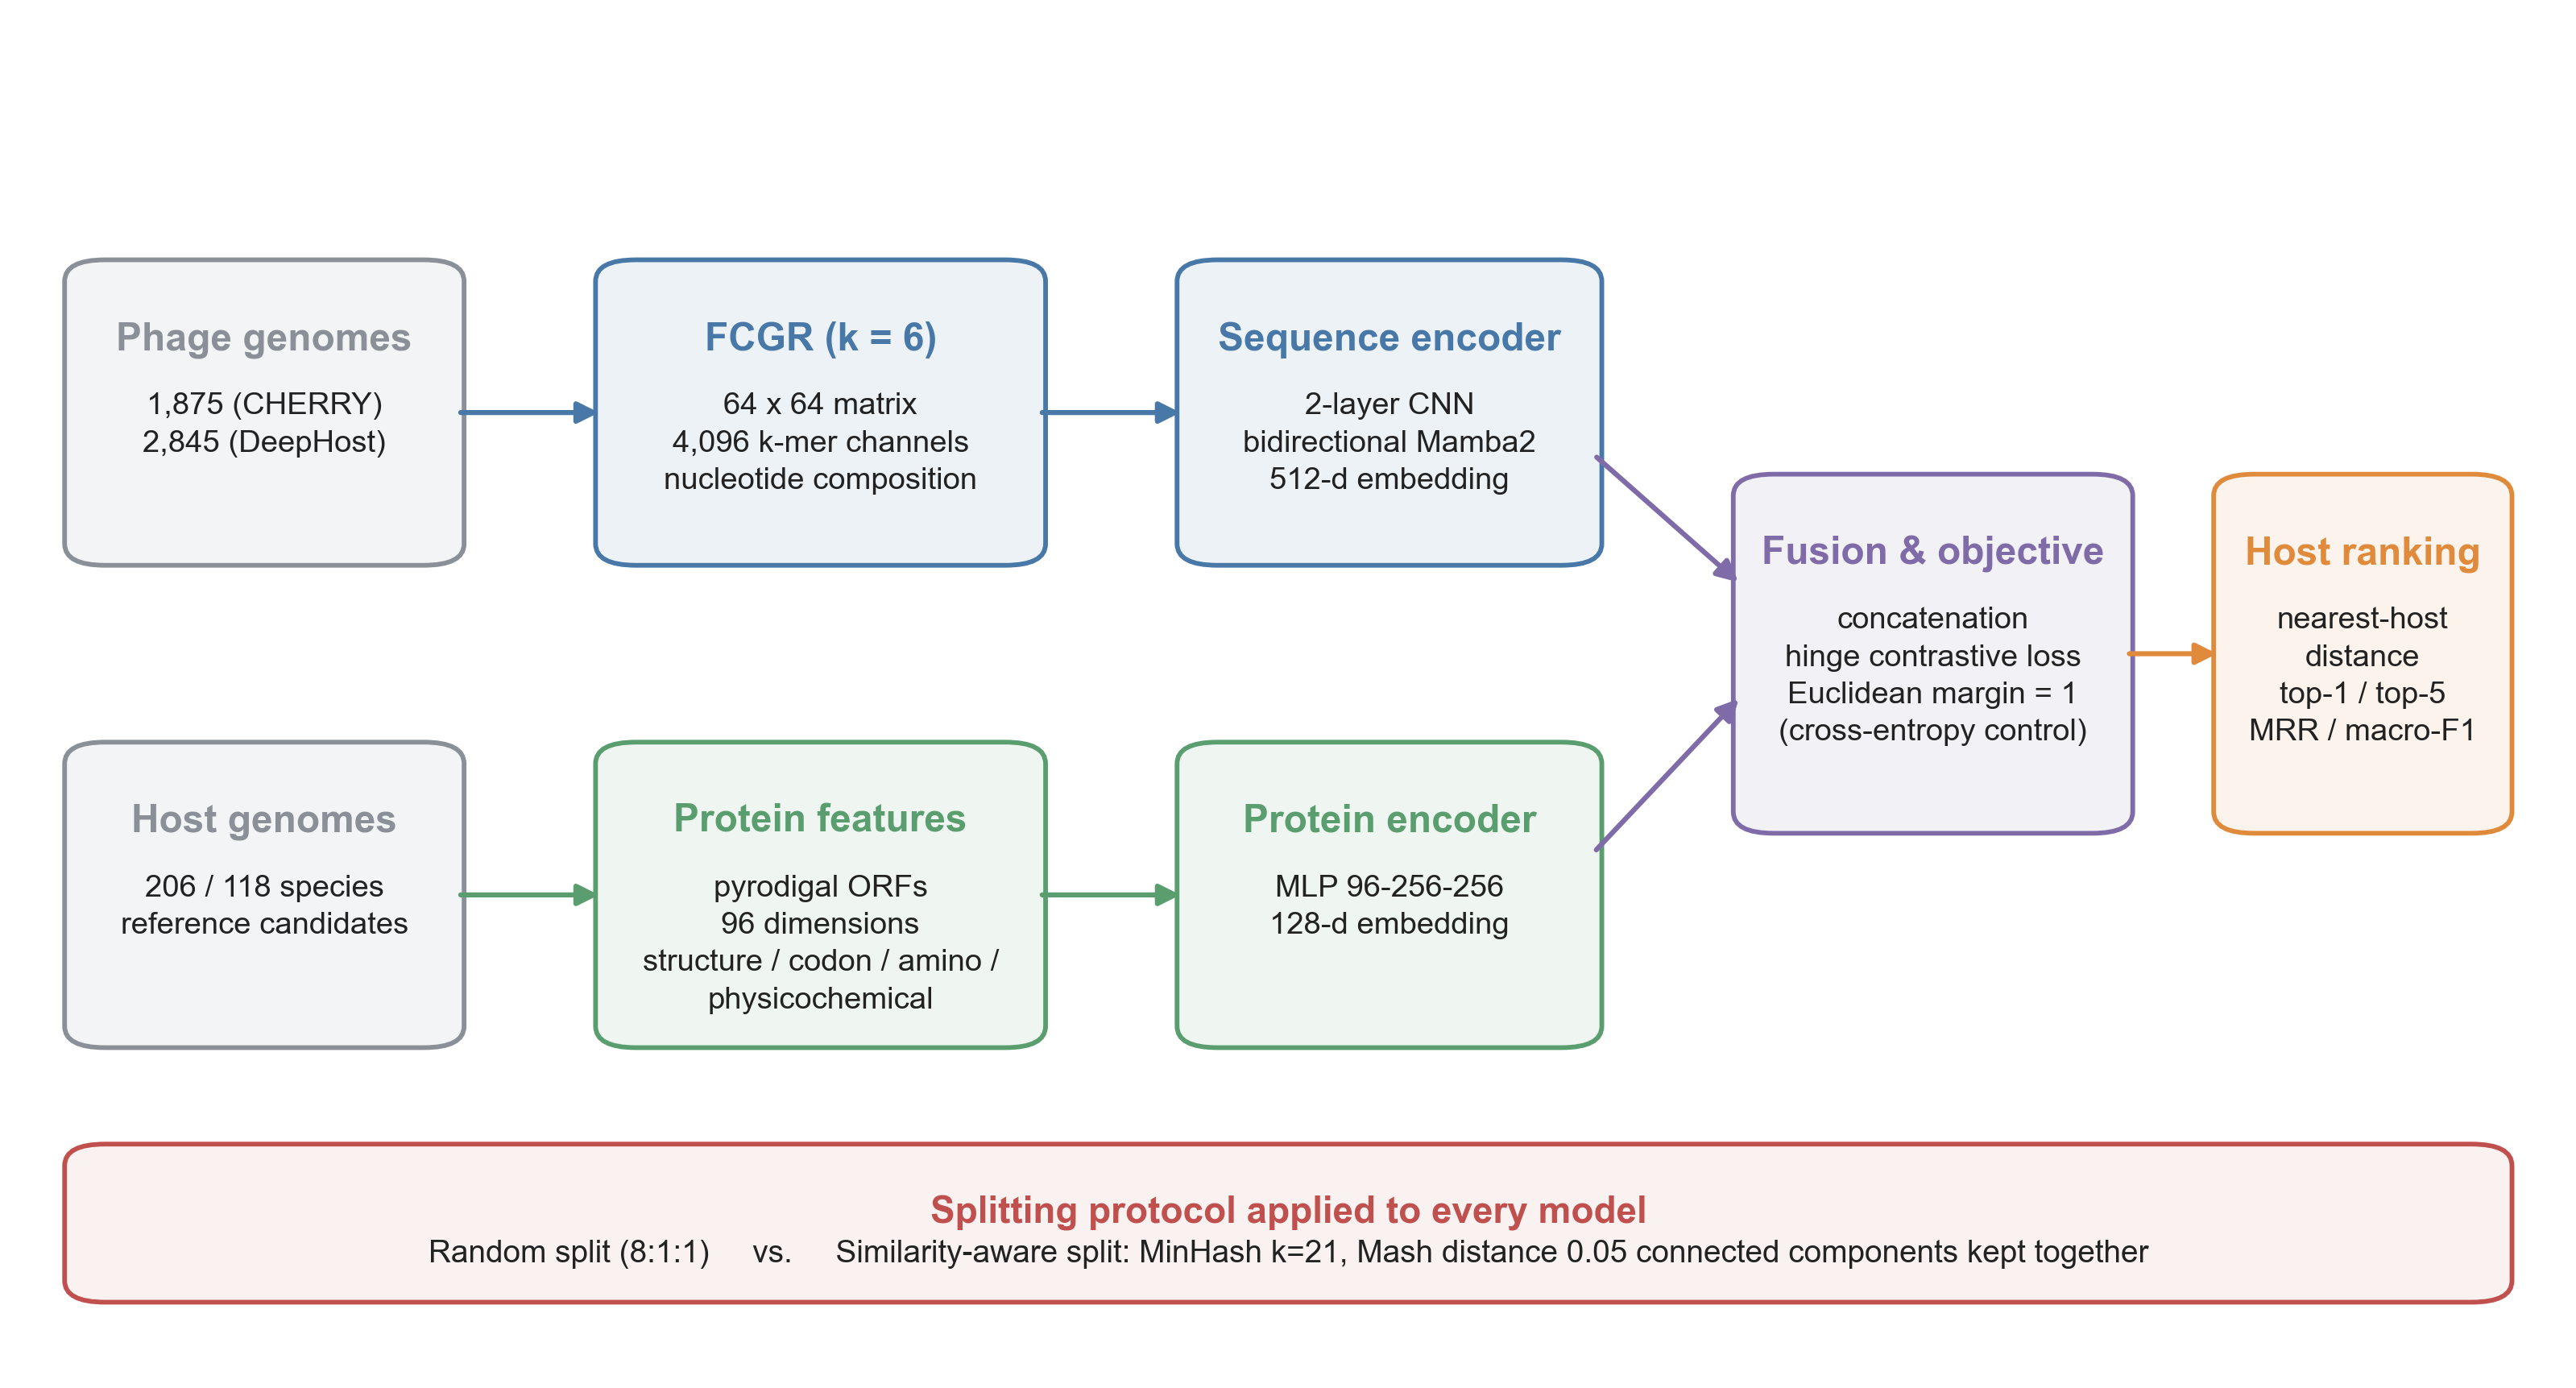
\includegraphics[width=\textwidth]{fig1_workflow.png}
\caption{End-to-end workflow. The five stages link curation and data audit, sequence and ORF-derived coding representations, the shared encoders, the two independent training pipelines, and the evaluation and statistical controls; the bottom band shows the random and similarity-aware split allocation.}
\label{fig:1}
\end{figure}

\begin{figure}[ht]
\centering
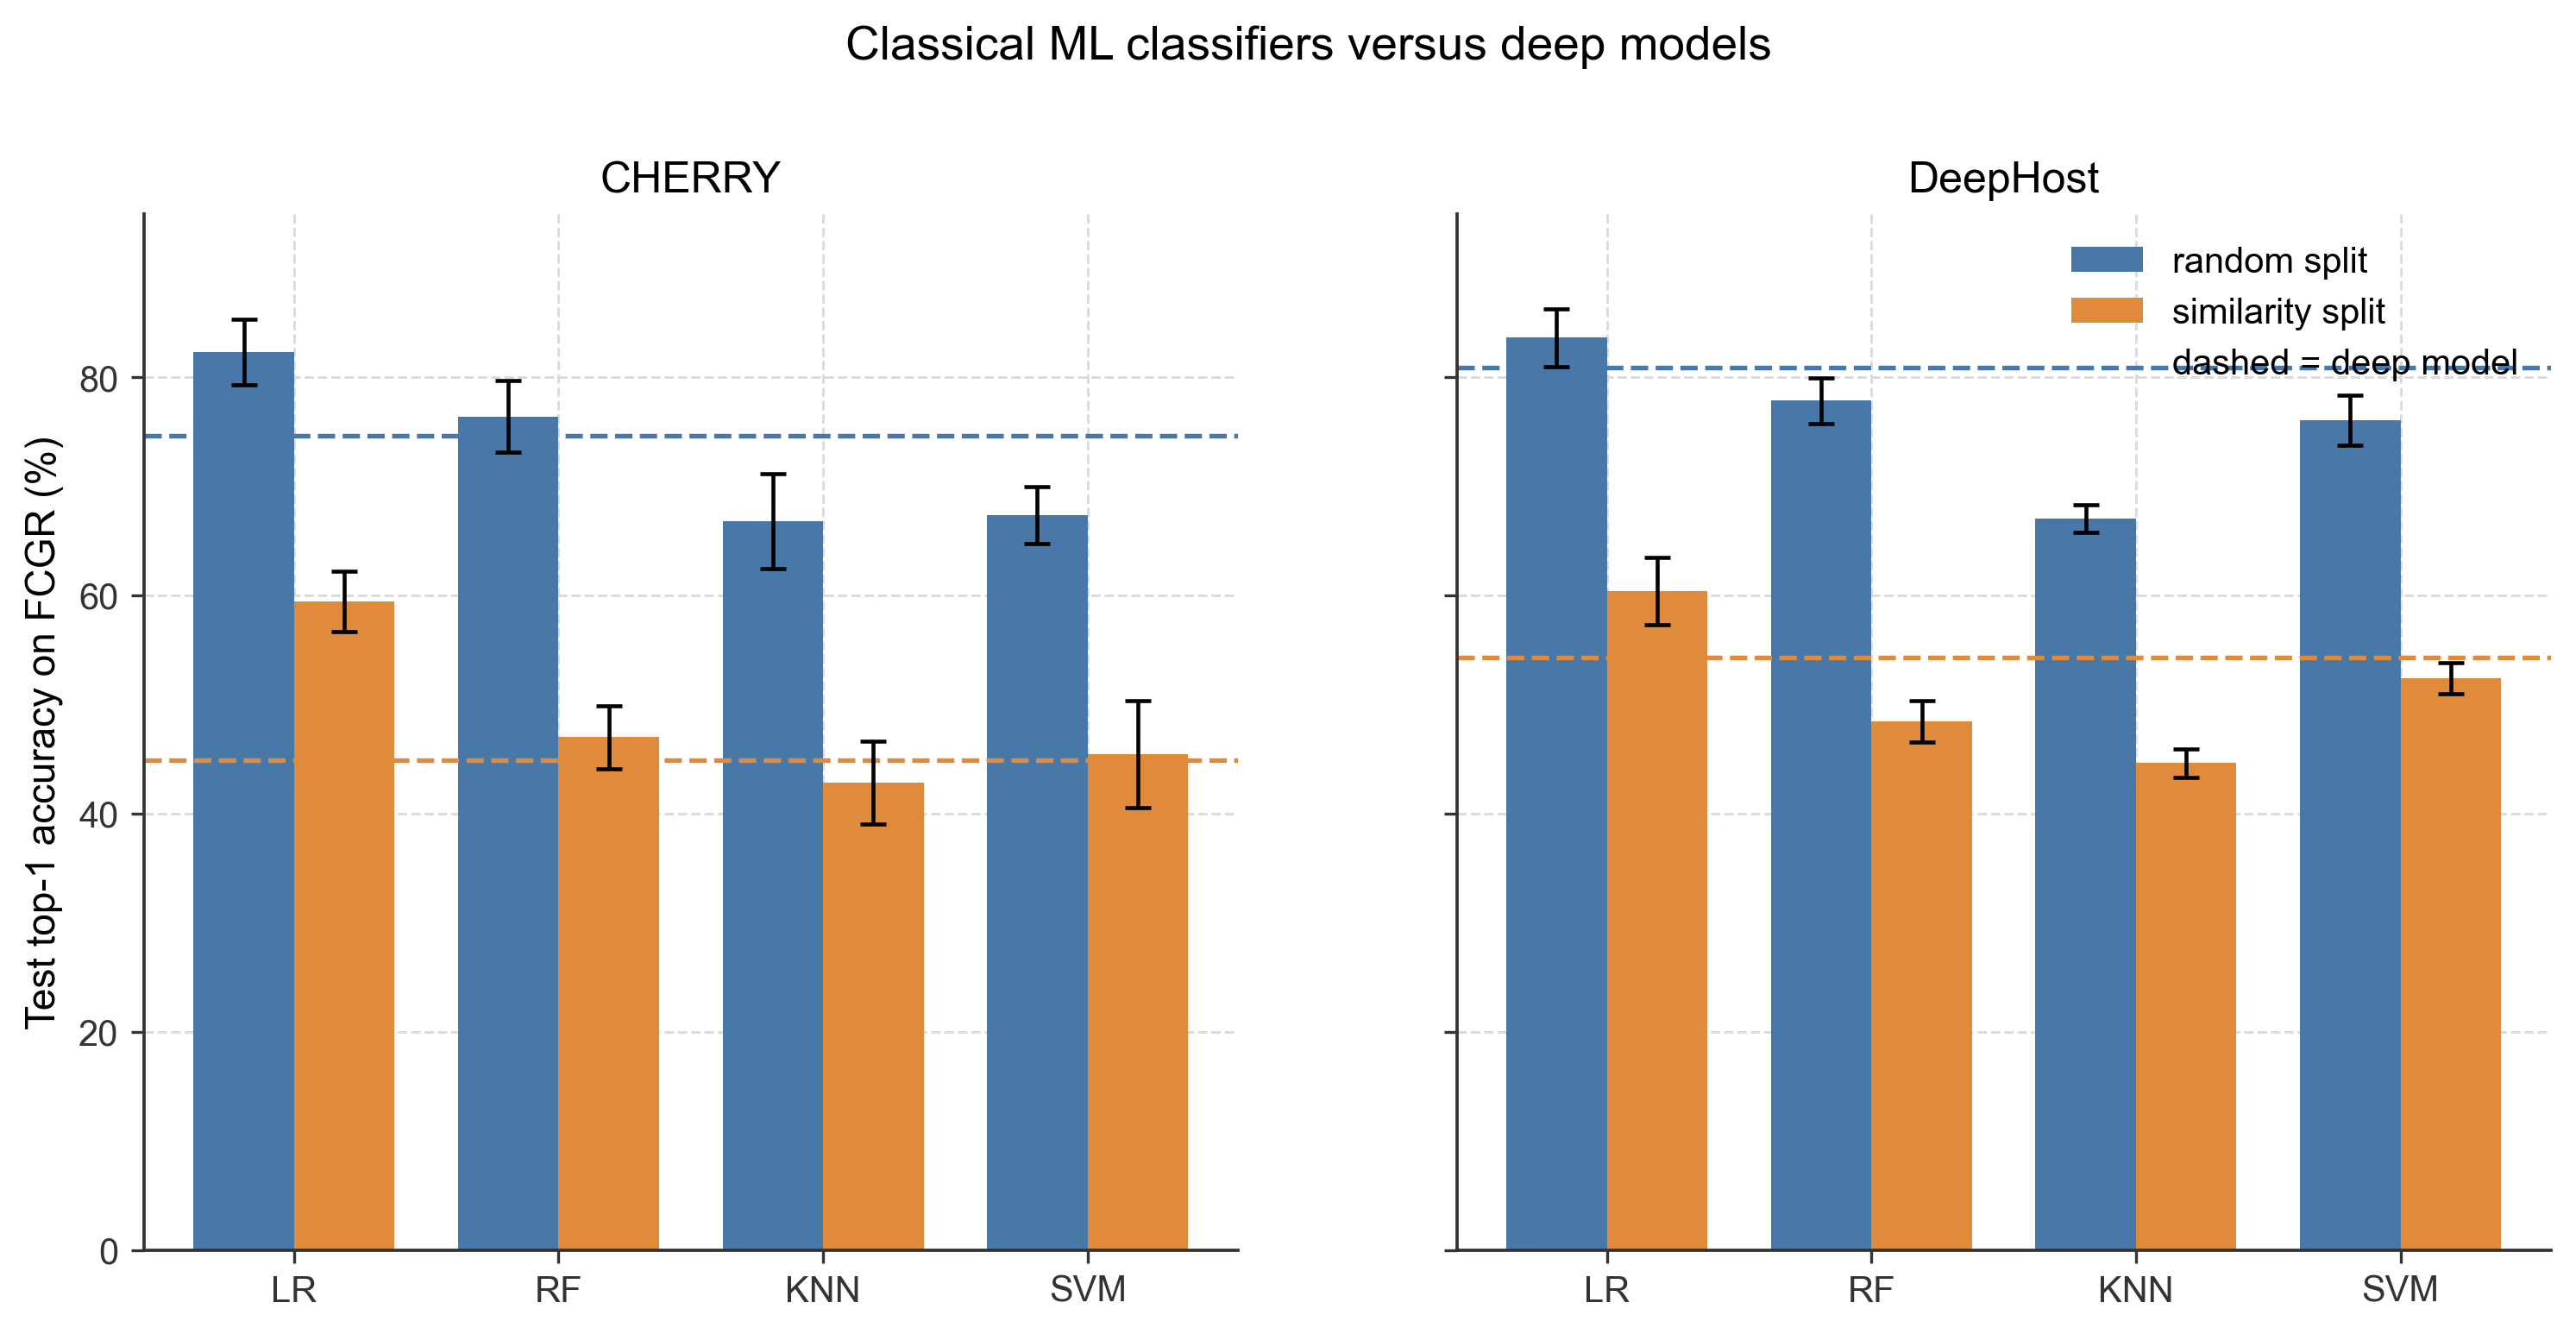
\includegraphics[width=0.92\textwidth]{fig2_ml.png}
\caption{Classical classifiers on FCGR under the random and similarity splits, with deep-model reference lines, on CHERRY and DeepHost (mean $\pm$ SD).}
\label{fig:2}
\end{figure}

\begin{figure}[ht]
\centering
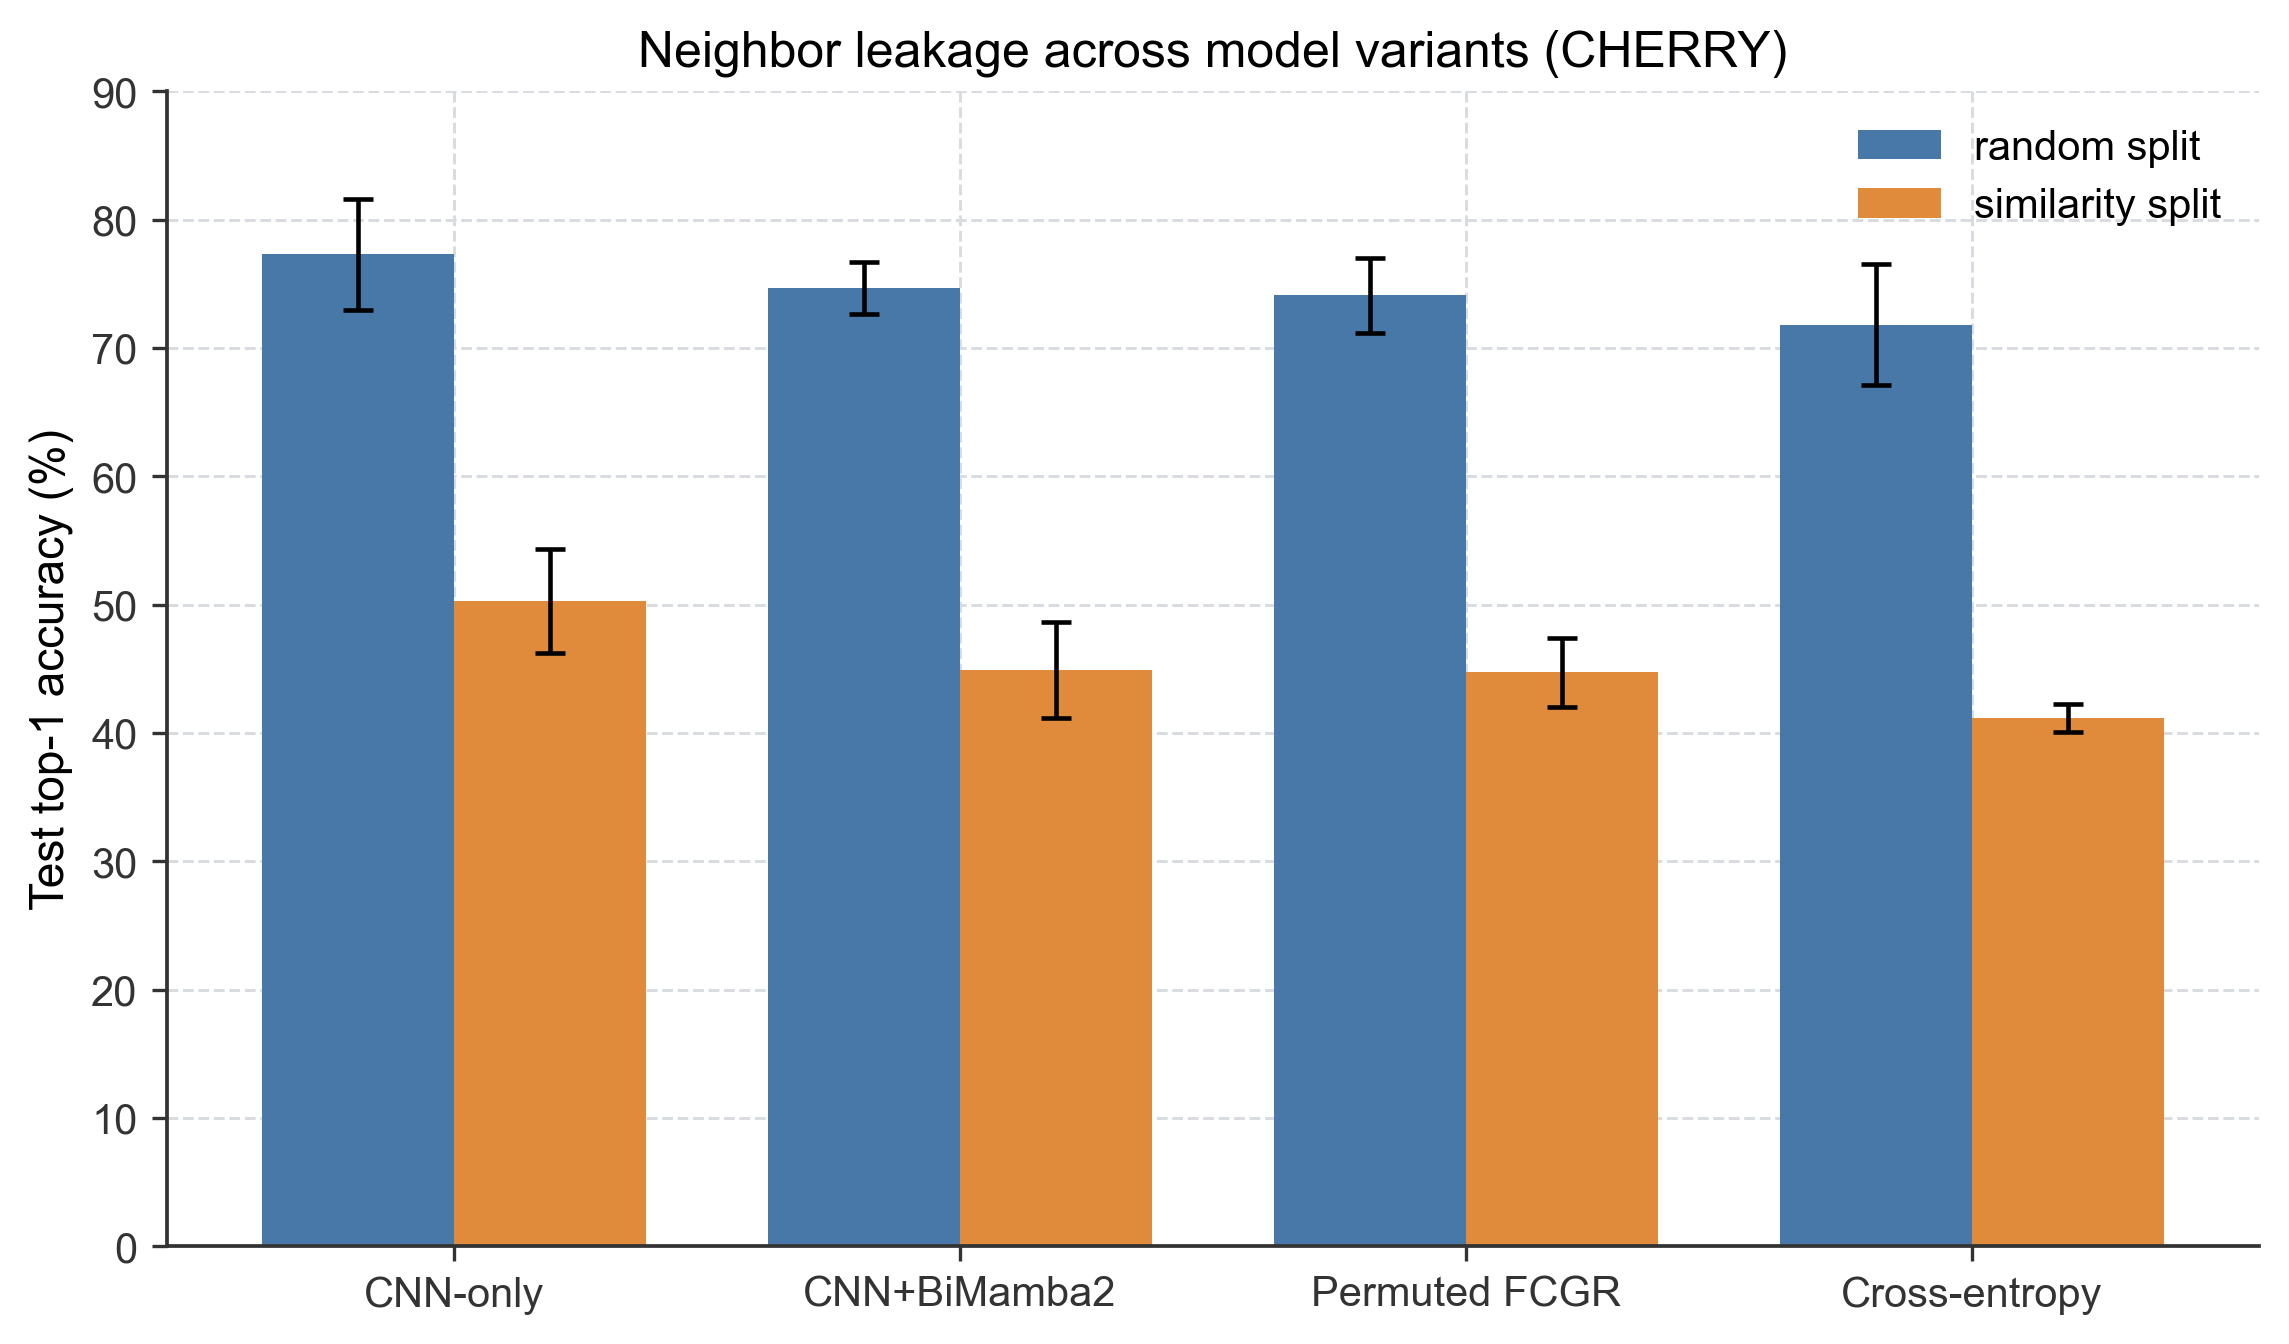
\includegraphics[width=0.92\textwidth]{fig3_leakage.png}
\caption{Top-1 accuracy of the deep sequence models under the random and similarity splits (mean $\pm$ SD), CHERRY.}
\label{fig:3}
\end{figure}

\begin{figure}[ht]
\centering
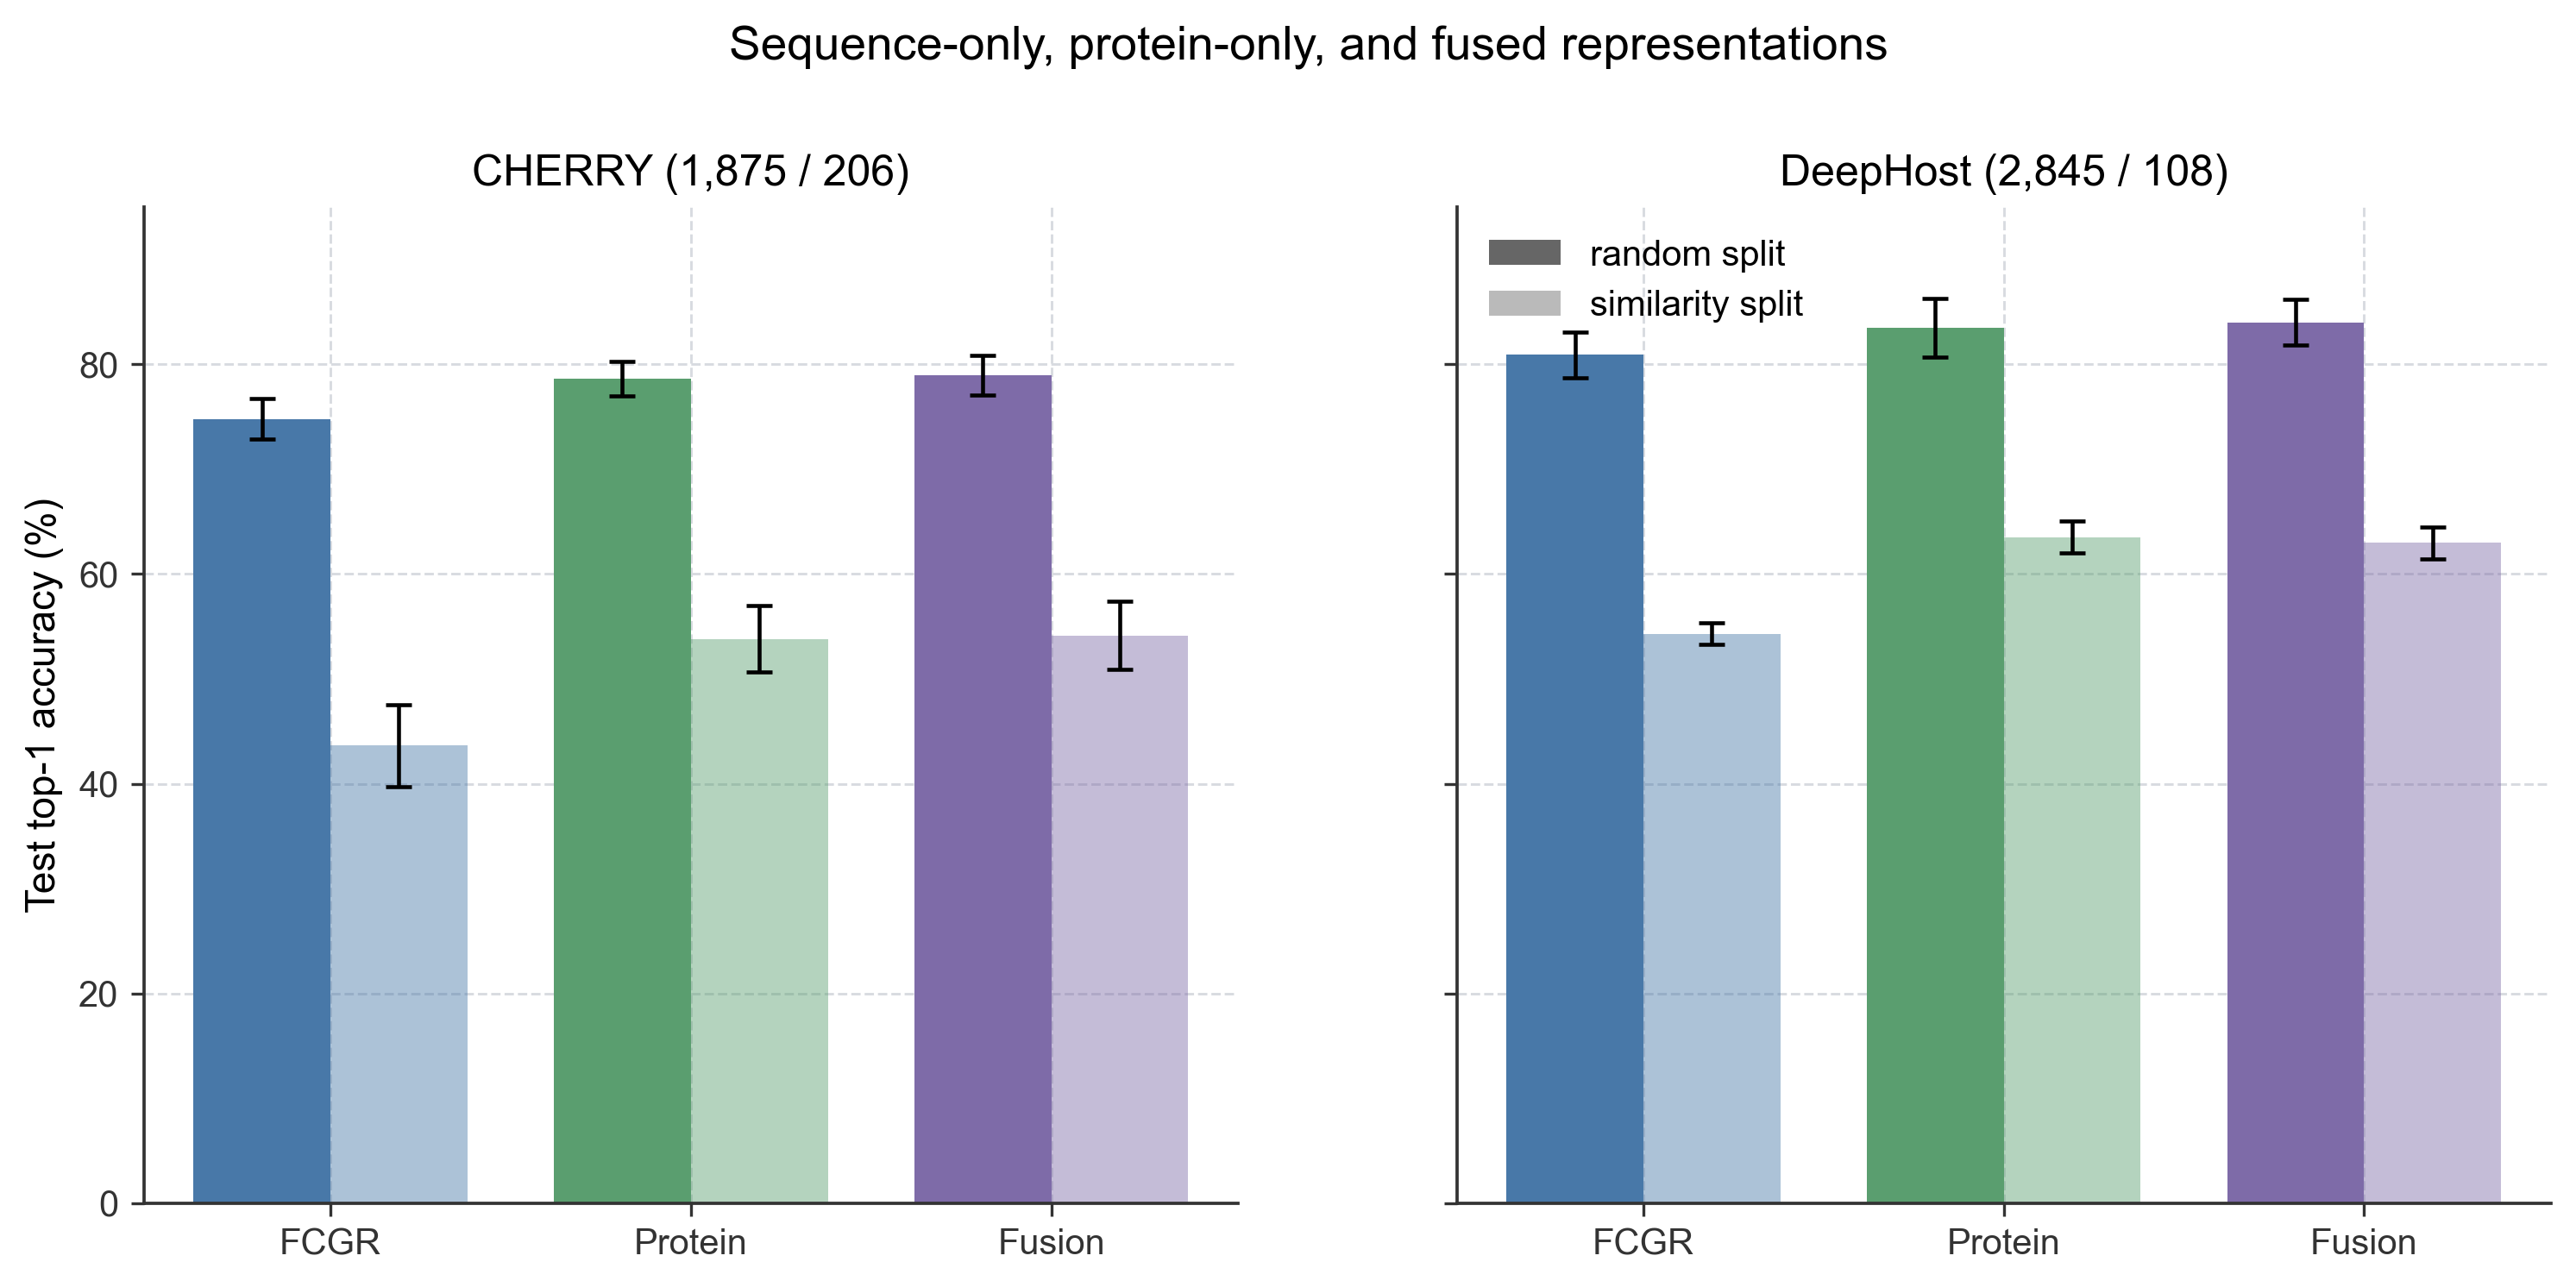
\includegraphics[width=0.92\textwidth]{fig5_protein.png}
\caption{Sequence-only, coding-only, and fusion variants under the two splits on CHERRY and DeepHost (mean $\pm$ SD, n=5).}
\label{fig:4}
\end{figure}

\begin{figure}[ht]
\centering
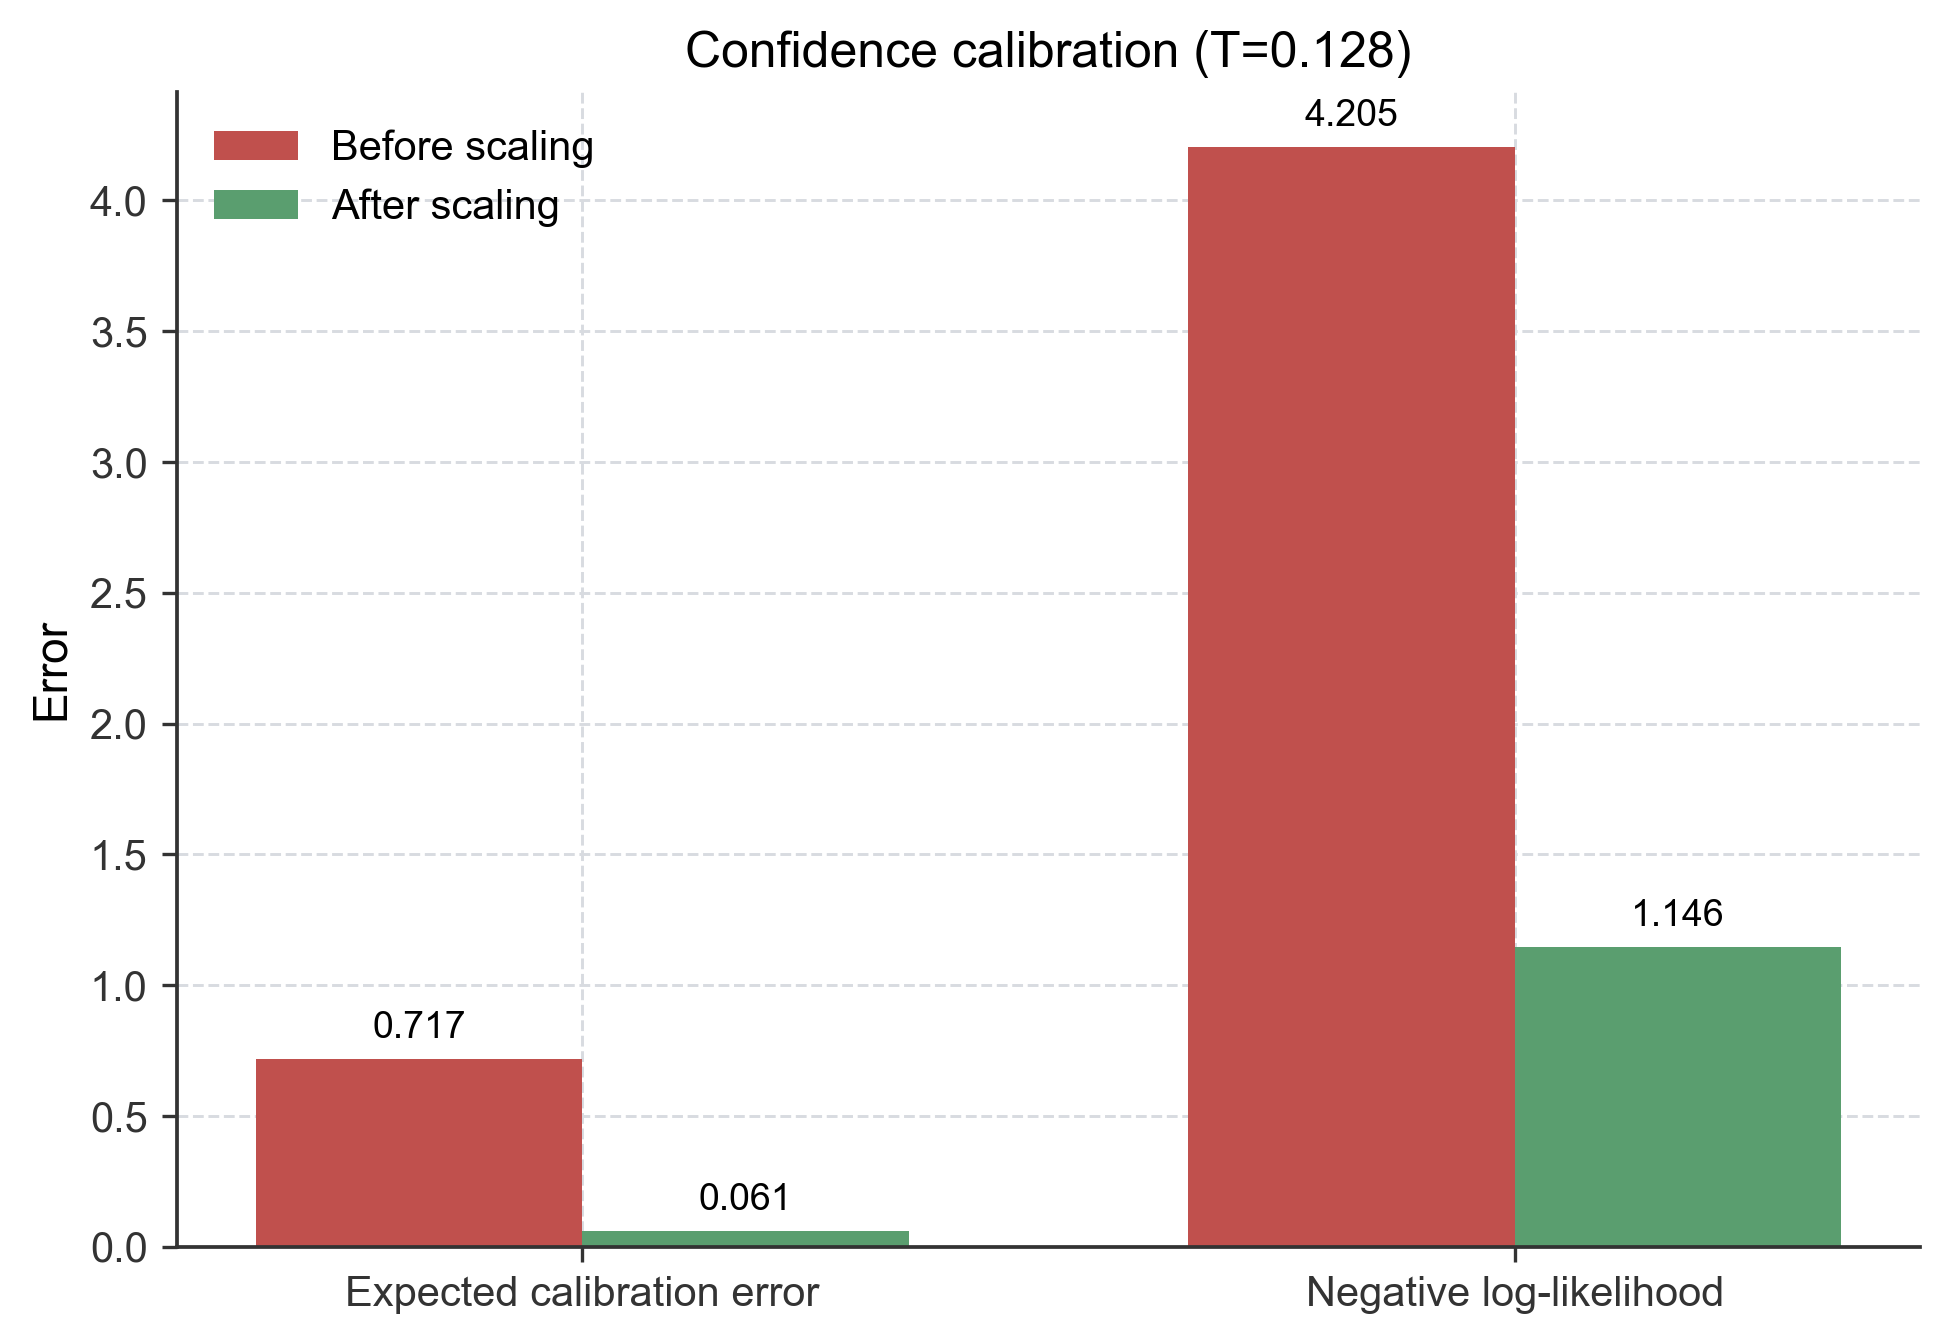
\includegraphics[width=0.85\textwidth]{fig7_calibration.png}
\caption{Expected calibration error and negative log-likelihood before and after temperature scaling (mean $\pm$ SD).}
\label{fig:5}
\end{figure}

\begin{figure}[ht]
\centering
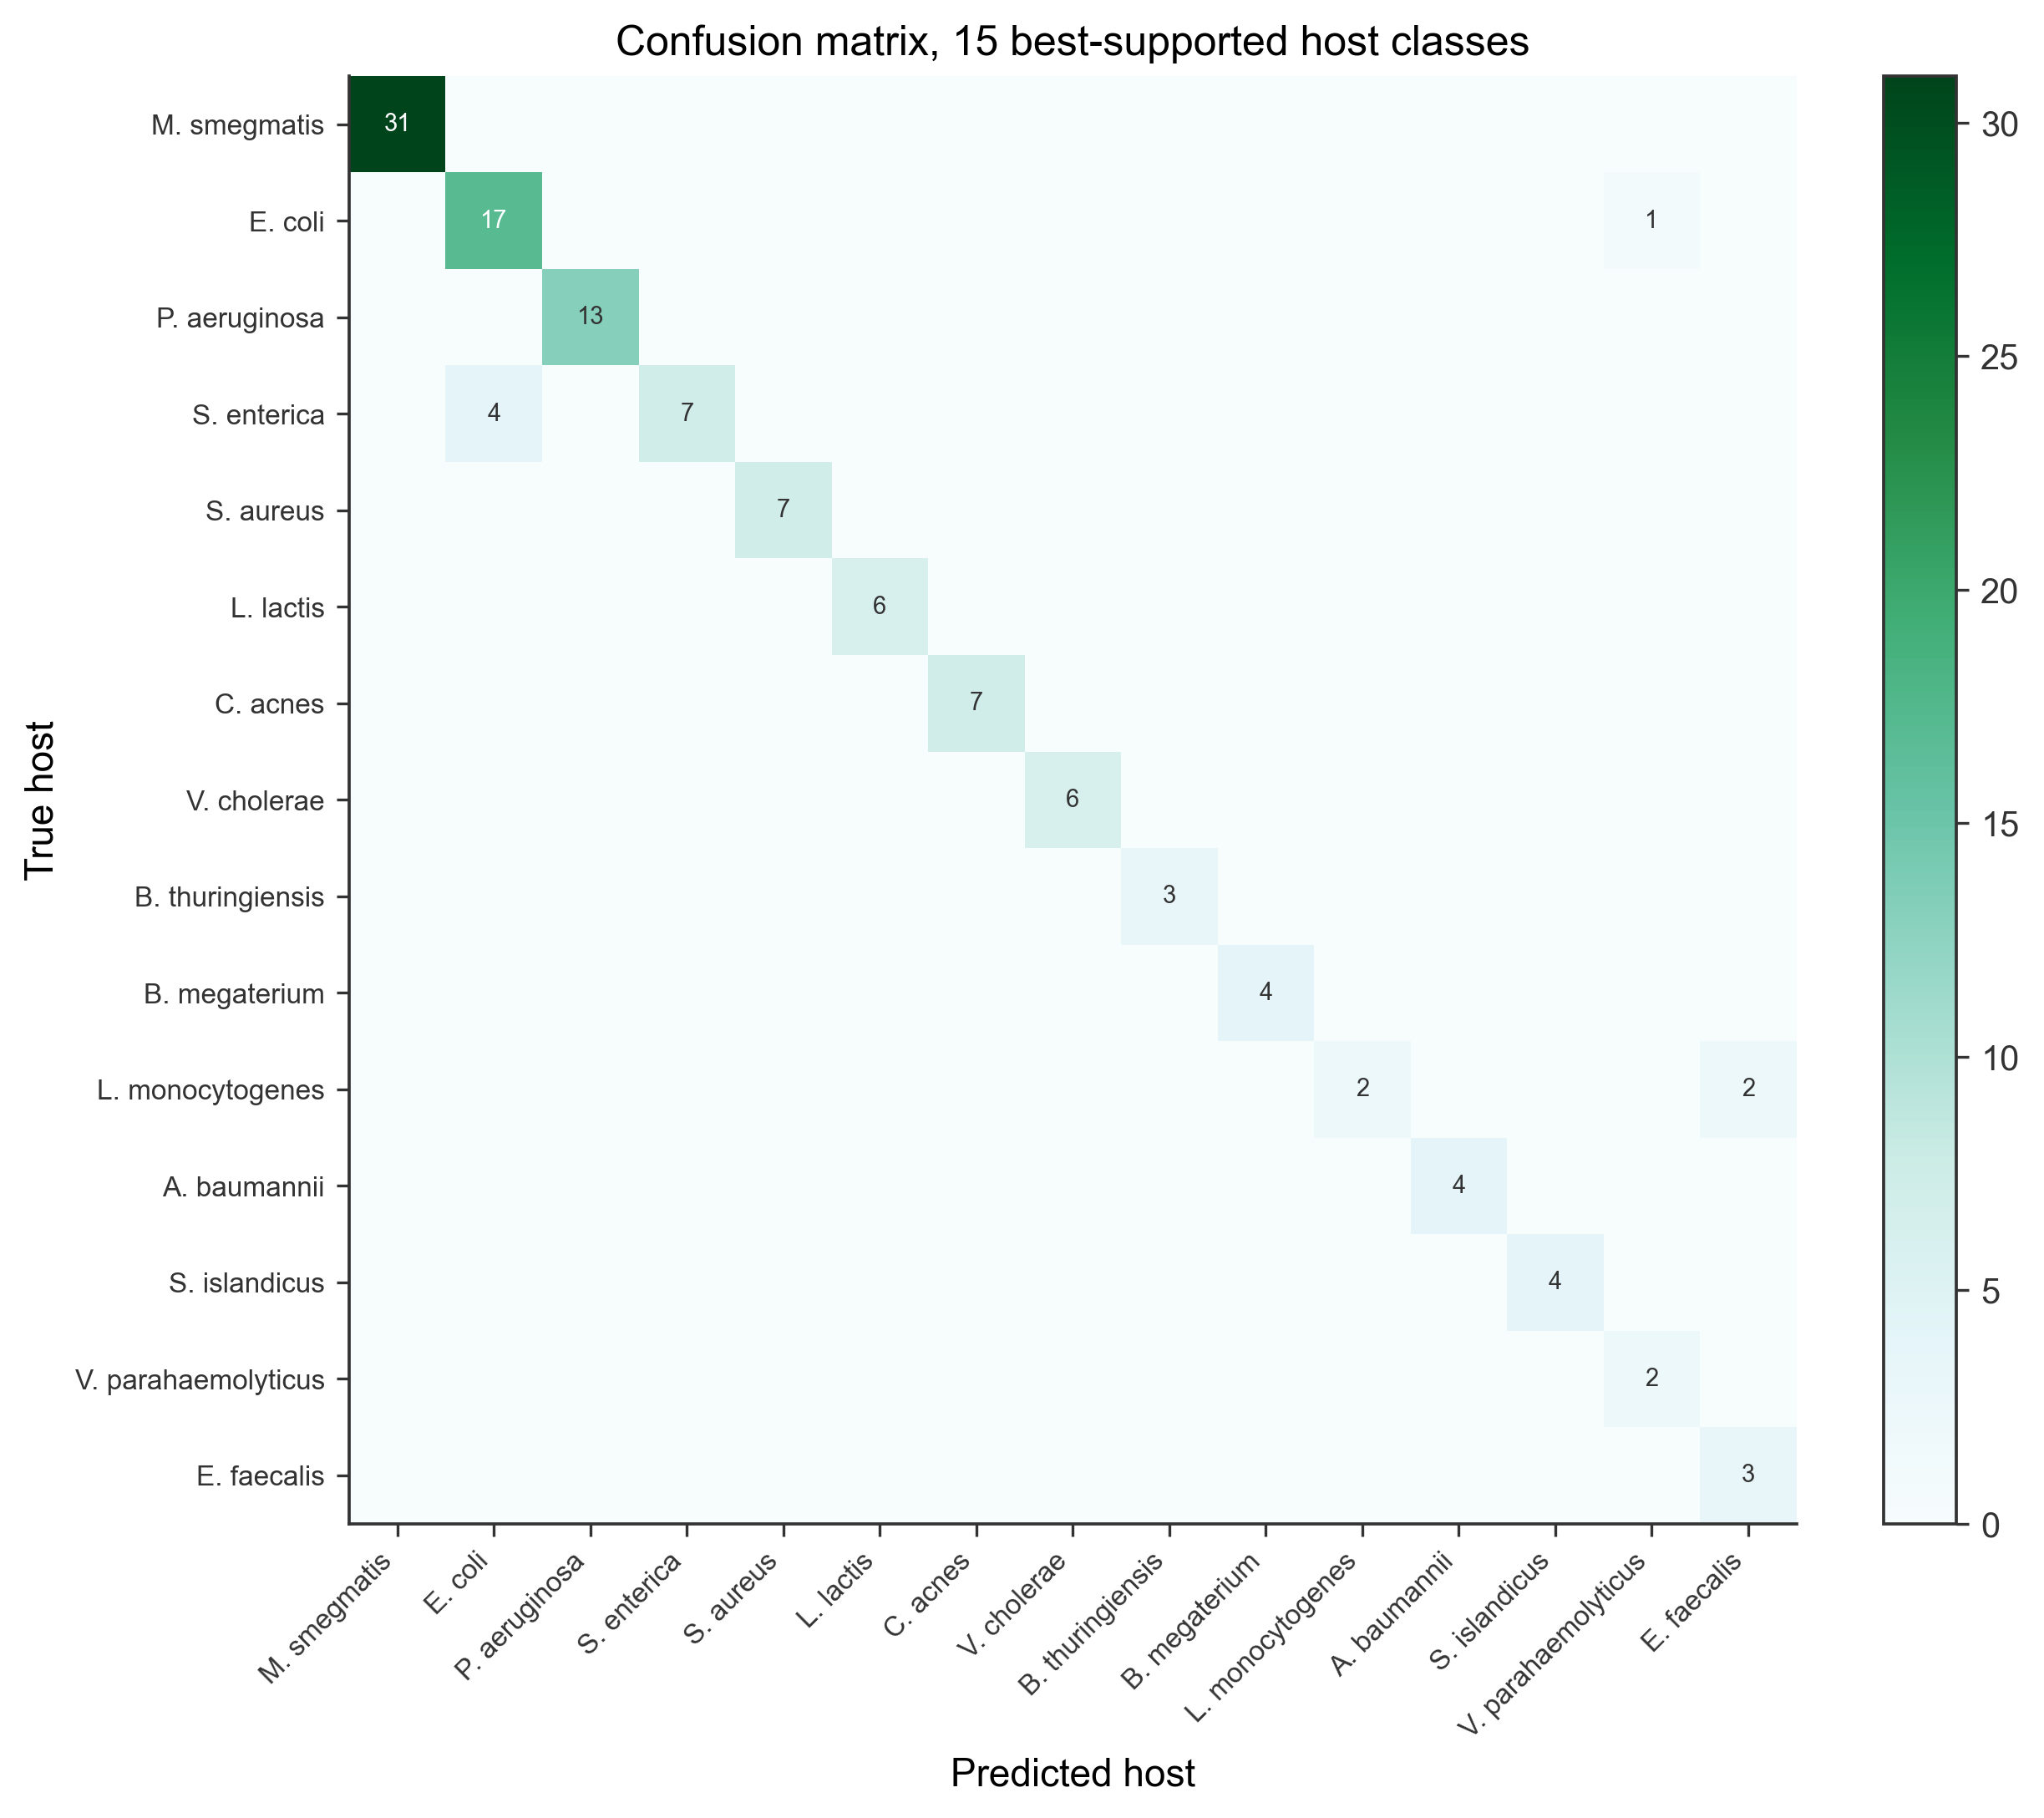
\includegraphics[width=0.9\textwidth]{fig8_confusion.png}
\caption{Confusion matrix for the 15 best-supported host classes on the seed-123 random split; the matrix is largely diagonal and residual errors concentrate among related hosts.}
\label{fig:6}
\end{figure}

\end{document}
